%%%%%%%%%%%%%%%%%%%%%%%%%%%%%%%%%%%%%%%%%%%%%%%%%%%%%%%%%%%%%
%% Isolated DC-DC converters %%
%%%%%%%%%%%%%%%%%%%%%%%%%%%%%%%%%%%%%%%%%%%%%%%%%%%%%%%%%%%%%
\section{Isolated DC-DC converters}

%%%%%%%%%%%%%%%%%%%%%%%%%%%%%%%%%%%%%%%%%%%%%%%%%%%%%%%%%%%%%
%% Some fundamentals %%
%%%%%%%%%%%%%%%%%%%%%%%%%%%%%%%%%%%%%%%%%%%%%%%%%%%%%%%%%%%%%
\subsection{Some fundamentals}

%%%%%%%%%%%%%%%%%%%%%%%%%%%%%%%%%%%%%%%%%%%%%%%%%%%%%%%%%%%%%
%% Galvanic isolation %%
%%%%%%%%%%%%%%%%%%%%%%%%%%%%%%%%%%%%%%%%%%%%%%%%%%%%%%%%%%%%%
\begin{frame}
    \frametitle{Galvanic isolation}
    \begin{columns}
        \begin{column}{0.5\textwidth}
             \begin{varblock}{A definition}
                Galvanic isolation is a principle of isolating functional sections of electrical circuits to prevent a direct current flow from input to output, that is, enabling different ground potentials for the circuit sections.   
             \end{varblock}%
             \vspace{1em}
        Typical reasons for requiring galvanic isolation are:
        \begin{itemize}
            \item Safety (prevention of electric shock),
            \item Noise reduction,
            \item contact corrosion reduction.
        \end{itemize}
        \end{column}
        \begin{column}{0.5\textwidth}
            \vspace{-0.75cm}
            \begin{figure}
                \begin{subfigure}{\textwidth} 
                    \begin{circuitikz}
                        \ctikzset{blocks/scale=2, block lateral anchors pos=0.7}
                        \path (0,0) node[twoportsplitshape](dcdc){} ; 
                        \draw (dcdc.left up) -- ++(-1,0) coordinate (A1) 
                        (dcdc.left down) to [short, -*] ++(-1,0) coordinate (A2)
                        (A1) to [V, v_=$u_1$] (A2)
                        (dcdc.right up) to [short, -o]  ++(1,0) coordinate (B1)
                        (dcdc.right down) to [short, -o] ++(1,0) coordinate (B2);
                        \draw (B1) to [open, v^=$u_2$, voltage = straight] (B2);
                        \path (3.25,0) node[graduate,mirrored,sword,minimum size=1.5cm, stripes = uniblue] (human){};
                        \draw (human.south) node[ground](G2){}
                        let \p1 = (G2), \p2 = (A2) in (\x2, \y1) node[ground](G1){}
                        (G1) -- (A2);
                        \draw let \p1 = (G2), \p2 = (A2)  in (\x2, \y1) [signalred, ultra thick, -latex, dashed] (G1.south) -- (\x2,\y2) -- (\x1,\y2) -- (G2.south) -- (G1.south);
                        \draw let \p1 = (G2), \p2 = (A2)  in (\x2/2+\x1/2, \y1) node[signalred, below] {current through ground};
                    \end{circuitikz}
                \caption{Lack of galvanic isolation}
            \end{subfigure}
            \begin{subfigure}{\textwidth} 
                \begin{circuitikz}
                    \ctikzset{blocks/scale=2, block lateral anchors pos=0.7}
                    \path (0,0) node[twoportsplitshape](dcdc){} ; 
                    \draw (dcdc.left up) -- ++(-1,0) coordinate (A1) 
                    (dcdc.left down) to [short, -*] ++(-1,0) coordinate (A2)
                    (A1) to [V, v_=$u_1$] (A2)
                    (dcdc.right up) to ++(0.15,0) node[transformer, anchor=A1, scale=0.655](T){}
                    (T.A2) -- (dcdc.right down)
                    (T.B1) to [open, v^=$u_2$, voltage = straight, o-o] (T.B2);
                    \path (3.7,0) node[graduate,mirrored,sword,minimum size=1.5cm, stripes = uniblue] (human){};
                    \draw (human.south) node[ground](G2){}
                    let \p1 = (G2), \p2 = (A2) in (\x2, \y1) node[ground](G1){}
                    (G1) -- (A2);
                    \draw [signalgreen, ultra thick, latex-latex, dashed] (G1.south) (G2.south) -- (G1.south);
                    \draw let \p1 = (G2), \p2 = (A2)  in (\x2/2+\x1/2, \y1) node[signalgreen, below] {output $u_2$ can 'float'};
                \end{circuitikz}
                \caption{Galvanic isolation via inductive separation}
            \end{subfigure}
                \caption{Why galvanic isolation can be useful}
                \label{fig:galvanic-isolation}
            \end{figure}
        \end{column}
    \end{columns}
\end{frame}

%%%%%%%%%%%%%%%%%%%%%%%%%%%%%%%%%%%%%%%%%%%%%%%%%%%%%%%%%%%%%
%% Galvanic isolation: technical realization %%
%%%%%%%%%%%%%%%%%%%%%%%%%%%%%%%%%%%%%%%%%%%%%%%%%%%%%%%%%%%%%
\begin{frame}
    \frametitle{Galvanic isolation: technical realization}
    \begin{table}
		\centering
		\begin{tabular}{M{0.3\textwidth} M{0.3\textwidth} M{0.3\textwidth}}
			\onslide<1->{Capacative} & \onslide<2->{Optical} & \onslide<3->{Inductive}\\[1em]

			\onslide<1->{
			\begin{circuitikz}
				\draw (0,-0.5) to [capacitor] (2,-0.5)
                (0,0.5) to [capacitor] (2,0.5);
			\end{circuitikz}
			}

			&
			\onslide<2->{
			\begin{circuitikz}
				\draw (0,0.5) to [empty photodiode, mirror] (2,0.5)
                (0,-0.5) to [empty led] (2,-0.5);
			\end{circuitikz}
			}
			
			&
			\onslide<3->{
			\begin{circuitikz}
				\draw (0,0) node[transformer](){};
			\end{circuitikz}
			}
            
            \\[1em]  
            
            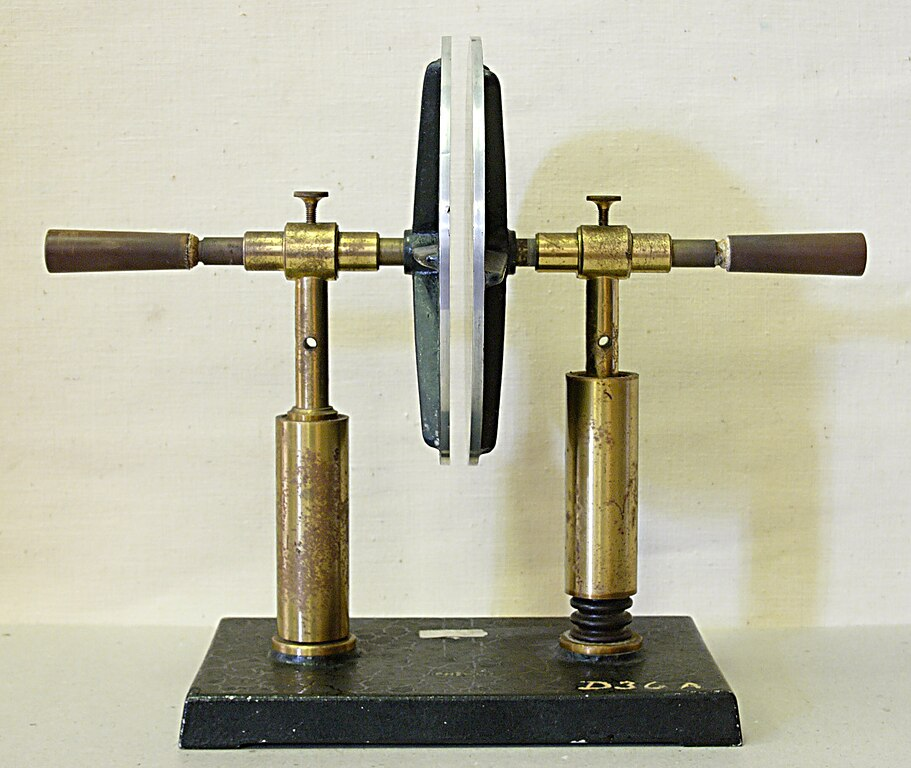
\includegraphics[height=0.25\textheight]{fig/lec03/Capacitor_example.jpg}
            
            {\small source: \href{https://commons.wikimedia.org/wiki/File:Plattenkondensator_hg.jpg}{Wikimedia Commons}, H.~Grobe, \href{https://creativecommons.org/licenses/by/3.0/deed.en}{CC~BY~3.0}}

            &

            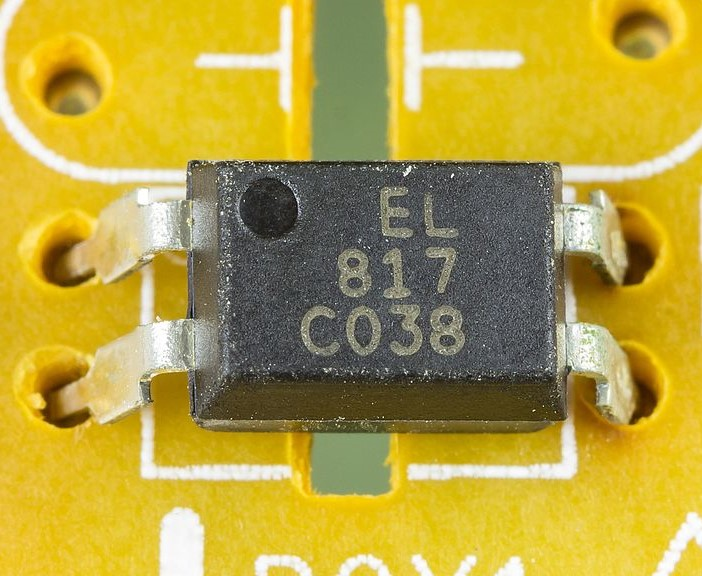
\includegraphics[height=0.25\textheight]{fig/lec03/Optocoupler_example.jpg}

            {\small source: \href{https://en.wikipedia.org/wiki/File:Philips_BDP3280-12_-_Everlight_EL817_on_power_board-1779.jpg}{Wikimedia Commons}, R.~Spekking, \href{https://creativecommons.org/licenses/by-sa/4.0/deed.en}{CC~BY-SA~4.0}}

            &
            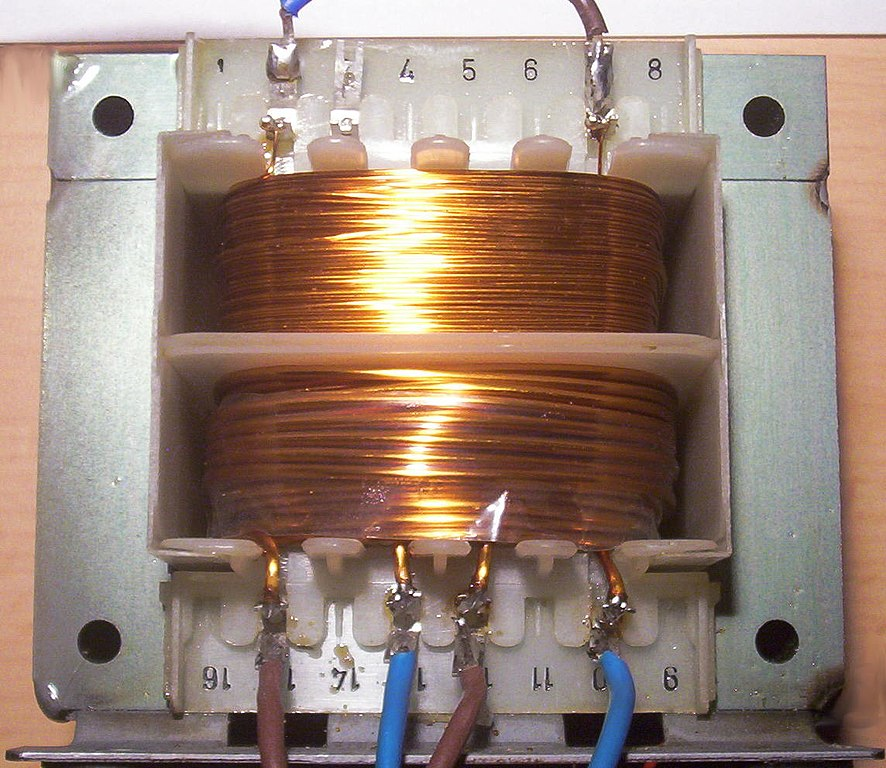
\includegraphics[height=0.25\textheight]{fig/lec03/Transformer_example.jpg}

            {\small source: \href{https://commons.wikimedia.org/wiki/File:Trafo-innenleben.jpg}{Wikimedia Commons}, S.~Riepl, public domain}

		\end{tabular}
	\end{table}
\end{frame}

%%%%%%%%%%%%%%%%%%%%%%%%%%%%%%%%%%%%%%%%%%%%%%%%%%%%%%%%%%%%%
%% Galvanic isolation via transformer %%
%%%%%%%%%%%%%%%%%%%%%%%%%%%%%%%%%%%%%%%%%%%%%%%%%%%%%%%%%%%%%
\begin{frame}
    \frametitle{Galvanic isolation via transformer}
    \begin{columns}
        \begin{column}{0.4\textwidth}
            \begin{itemize}
                \item In power electronics, transformers are mostly used to provide galvanic isolation.
                \item Reason: the power density per volume and weight is typically higher than for capacitive or optical isolation.
                \item Assumptions for the following model:
                \begin{itemize}
                    \item Ideal coupling \newline(no leakage flux),
                    \item no losses,
                    \item no saturation.
                \end{itemize}
            \end{itemize}
        \end{column}
        \begin{column}{0.6\textwidth}
            \begin{figure}
                \begin{tikzpicture}[global scale/.style={scale=1.0}, rotate=-5, xslant=-0.1, thick, every
                    node/.style={transform shape, scale=0.8}, decoration={markings, mark=at position 0.5 with {\arrow{latex}}}]
                    \tikzmath{
                        real \a, \b, \dx, \dy, \lx, \ly, \dr;
                        \a = 3.0;
                        \b = 5.0;
                        \dx = 0.8;
                        \dy = 0.5;
                        \lx = 1.0;
                        \ly = 1.0;
                        \dr = 0.02;
                    } 
                    \begin{scope}[even odd rule, scale=0.9]
                    \filldraw[rounded corners=2pt, fill=gray, rotate=-0, opacity=1.0] (\dx,
                    \dy) rectangle ++(5,5) (\lx+\dx,\ly+\dy) rectangle ++(\a, \a);
                    \fill [rounded corners=2pt, fill=gray] (\b, 0) --++ (0, \dy+\dr+0.02) --++(\dx, 0) --cycle;
                    \fill [rounded corners=2pt, fill=gray] (0, \b) --++ (\dx+\dr+0.02, 0) --++(0, \dy)--cycle;
                    \filldraw[rounded corners=2pt, fill=gray!50, rotate=-0] (0,0) rectangle
                    ++(\b, \b) (\lx,\ly) rectangle ++(\a, \a);
                    \draw (\b-\dr,\dr) --++(\dx, \dy);
                    \draw (\b-\dr,\b-\dr) --++(\dx, \dy);
                    \draw (\dr,\b-\dr) --++(\dx, \dy);
                    \draw [signalblue, thick, postaction={decorate}] (0, \ly) --++(-1.5,0);
                    \draw [rounded corners=2pt,signalblue, thick]
                        (-0.09,\ly) -- (\lx, \ly)--++(0.89,0.5)
                        --++(-0.08, 0.05);
                    \foreach \z in {.24,.48,...,2.5}
                        {
                        \draw [rounded corners=2pt,signalblue, thick]
                        (-0.0,\ly+\z+0.08)--(-0.09,\ly+\z) -- (\lx, \ly+\z)--++(0.89,0.5)
                        --++(-0.08, 0.05);
                    }
                    \draw [rounded corners=2pt,signalblue, thick, postaction={decorate}] (-1.5,
                    \ly+2.8) --++(1.5,0) node[black, above, pos=0.4] {$i_1(t)$};
                    \draw[latex-] (-\lx, \ly+0.2) --++(0, 2.4) node[midway, left] {$u_1(t)$};
                    
                    \draw [rounded corners=2pt,signalred, thick] (\a+\lx-2*\dr,
                    \ly+2*\dr)--++(-\dr, -\dr)--++(\lx+\dx+2*\dr, 0);
                    \draw [signalred, postaction={decorate}] (\b+\dx-\dr+\a/2, \ly+\dr)--(\b+\dx-\dr, \ly+\dr);
                    \draw [rounded corners=2pt, signalred, thick, postaction={decorate}]
                    (\a+3*\lx-0.2, \ly+3.1) --++(\a/2, 0) node[black, midway, above] {$i_2(t)$};
                    \foreach \z in {.125,.25,.375,...,2.5}
                        {
                        \draw [rounded corners=2pt, signalred, thick] (\a+\lx,\ly+\z+0.1)--
                        (\a+\lx-0.07,\ly+\z) -- (\a+2*\lx, \ly+\z)--++(0.87,0.5)--++(-0.06,
                        0.06);
                        }
                    \draw[latex-] (2*\a+\lx, \ly+0.25) --++(0, 2.6) node[midway, left] {$u_2(t)$};
                    \end{scope}
                \end{tikzpicture}
                \caption{Simple transformer with primary and secondary winding}
                \label{fig:transformer_pseudo_3D}
            \end{figure}
        \end{column}
    \end{columns}
\end{frame}

%%%%%%%%%%%%%%%%%%%%%%%%%%%%%%%%%%%%%%%%%%%%%%%%%%%%%%%%%%%%%
%% Simplistic transformer model %%
%%%%%%%%%%%%%%%%%%%%%%%%%%%%%%%%%%%%%%%%%%%%%%%%%%%%%%%%%%%%%
\begin{frame}
    \frametitle{Simplistic transformer model}
    \begin{figure}
        \begin{subfigure}{0.4\textwidth}
            \centering
            \begin{tikzpicture}
                \draw (0,0) node[transformer core](T){$N_1:N_2$}
                (T.inner dot A1) node[circ]{}
                (T.inner dot B1) node[circ]{}
                (T.A1) to [short, -o, i<_=$i_1(t)$] ++(-1,0) coordinate (A1)
                (T.A2) to [short, -o] ++(-1,0) coordinate (A2)
                (T.B1) to [short, -o, i=$i_2(t)$] ++(1,0) coordinate (B1)
                (T.B2) to [short, -o] ++(1,0) coordinate (B2);
                \draw (A1) to [open, v=$u_1$, voltage = straight] (A2)
                (B1) to [open, v^=$u_2$, voltage = straight] (B2);
                \draw[dashed, thin] let \p1=(T.A1), \p2=(T.B2) in (\x1 + 2mm,\y1 + 10mm) rectangle (\x2 - 2mm,\y2 - 12.5mm)
                (\x1/2 + \x2/2,\y1 + 10mm) node[above] {Transformer};
            \end{tikzpicture}
           \caption{Schematic symbol representation} 
        \end{subfigure}
        \begin{subfigure}{0.4\textwidth}
            \centering
            \begin{tikzpicture}
                \draw (0,0) node[transformer core](T){$N_1:N_2$}
                (T.inner dot A1) node[circ]{}
                (T.inner dot B1) node[circ]{}
                (T.A1) to [short, -*, i<_=$i'_1(t)$] ++(-1,0) coordinate (A1)
                (T.A2) to [short, -*] ++(-1,0) coordinate (A2)
                (A1) to [inductor, l=$L_\mathrm{m}$, i=$i_\mathrm{m}(t)$] (A2)
                (A1) to [short, -o, i<_=$i_1(t)$] ++(-1.5,0) coordinate (A11)
                (A2) to [short, -o] ++(-1.5,0) coordinate (A22)
                (T.B1) to [short, -o, i=$i_2(t)$] ++(1,0) coordinate (B1)
                (T.B2) to [short, -o] ++(1,0) coordinate (B2);
                \draw (A11) to [open, v=$u_1$, voltage = straight] (A22)
                (B1) to [open, v^=$u_2$, voltage = straight] (B2);
                \draw[dashed, thin] let \p1=(A1), \p2=(T.B2) in (\x1 - 3mm,\y1 + 10mm) rectangle (\x2,\y2 - 12.5mm)
                (\x1/2 + \x2/2 -2.5mm,\y1 + 10mm) node[above] {Transformer};
                \draw[dashed, thin] let \p1=(T.A1), \p2=(T.B2) in (\x1 + 2mm,\y1 + 5mm) rectangle (\x2 - 2mm,\y2 - 2.5mm)
                (\x1/2 + \x2/2,\y2 - 2.5mm) node[below, align=center] {Ideal\\ transformer};
            \end{tikzpicture}
            \caption{Equivalent circuit model} 
        \end{subfigure}
        \caption{Transformer model}
        \label{fig:transformer_model}
    \end{figure}
\end{frame}

%%%%%%%%%%%%%%%%%%%%%%%%%%%%%%%%%%%%%%%%%%%%%%%%%%%%%%%%%%%%%
%% Simplistic transformer model (cont.) %%
%%%%%%%%%%%%%%%%%%%%%%%%%%%%%%%%%%%%%%%%%%%%%%%%%%%%%%%%%%%%%
\begin{frame}
    \frametitle{Simplistic transformer model (cont.)}
    Based on \figref{fig:transformer_model} we consider the transformer as a combination of an ideal transformer with the conversion ratios
    \begin{equation}
        \frac{u_1(t)}{u_2(t)} = \frac{N_1}{N_2} \quad \text{and} \quad \frac{i'_1(t)}{i_2(t)} = \frac{N_2}{N_1}
    \end{equation}
    and an inductor with the magnetizing inductance $L_\mathrm{m}$:
    \begin{equation}
        u_1(t) = L_\mathrm{m} \frac{\mathrm{d}i_\mathrm{m}(t)}{\mathrm{d}t} \quad \text{and} \quad i_1(t) = i'_1(t) + i_\mathrm{m}(t).
    \end{equation}
    \begin{itemize}
        \item $L_\mathrm{m}$ models the magnetic energy stored in the transformer.
        \item Above model is a significant simplification (very first principle approach).
        \item More details on the transformer model can be found in the \href{https://github.com/IAS-Uni-Siegen/EMD_course}{Electrical Machines and Drives} course material.
    \end{itemize}
\end{frame}

%%%%%%%%%%%%%%%%%%%%%%%%%%%%%%%%%%%%%%%%%%%%%%%%%%%%%%%%%%%%%
%% Flyback converter %%
%%%%%%%%%%%%%%%%%%%%%%%%%%%%%%%%%%%%%%%%%%%%%%%%%%%%%%%%%%%%%
\subsection{Flyback converter}

%%%%%%%%%%%%%%%%%%%%%%%%%%%%%%%%%%%%%%%%%%%%%%%%%%%%%%%%%%%%%
%% Topology derivation based on the inverting buck-boost converter %%
%%%%%%%%%%%%%%%%%%%%%%%%%%%%%%%%%%%%%%%%%%%%%%%%%%%%%%%%%%%%%
\begin{frame}
    \frametitle{Topology derivation based on the inverting buck-boost converter}
    \begin{figure}
        \begin{circuitikz}[]
            \draw (0,0) to [short, *-] ++(1.0,0)
            to [diode, l=$D$, invert]  ++(1.0,0)
            to [short, -o, i=$i_2(t)$] ++(1.0,0)
            to [open, o-o, v = $\hspace{2cm}u_2(t)$, voltage = straight] ++(0,-2) coordinate (A)
            (0,0) to [short, *-] ++(-1.0,0) 
            to [Tnpn, n=npn1] ++(-1.0,0)
            to [short, -o, i_<=$i_1(t)$] ++(-1.0,0)
            to [open, o-o, v_= $u_1(t)\hspace{0.75cm}$, voltage = straight] ++(0,-2)
            to [short, o-o] (A)
            (0,0) to [inductor, *-*] ++(0,-2);
            \draw let \p1 = (npn1.B) in node[anchor=north] at (\x1,\y1) {$T$};
            \draw [decorate,decoration={brace,amplitude=10pt,mirror,raise=0.5cm},yshift=0pt] (-3,-2.0) -- (3,-2.0) node [black,midway,yshift=-0.6cm] {};
        \end{circuitikz}
        \begin{circuitikz}[]
            \draw (0,0) to [short] ++(1.0,0)
            to [diode, l=$D$, invert]  ++(1.0,0)
            to [short, -o, i=$i_2(t)$] ++(1.0,0)
            to [open, o-o, v = $\hspace{2cm}u_2(t)$, voltage = straight] ++(0,-2) coordinate (A)
            (0,0) to [short] ++(-1.0,0) 
            to [Tnpn, n=npn1] ++(-1.0,0)
            to [short, -o, i_<=$i_1(t)$] ++(-1.0,0)
            to [open, o-o, v_= $u_1(t)\hspace{0.75cm}$, voltage = straight] ++(0,-2)
            to [short, o-o] (A)
            (-0.5,0) to [inductor, *-*, n=l1] ++(0,-2)
            (0.5,0) to [inductor, *-*, n=l2, mirror] ++(0,-2);
            \draw let \p1 = (npn1.B) in node[anchor=north] at (\x1,\y1) {$T$};
            \path (l1.ul dot) node[circ]{}
                (l2.ul dot) node[circ]{};
            \draw (l1.midtap) node[left]{$N_1$}
            (l2.midtap) node[right]{$N_2$};
            \draw[double, double distance=3pt, thick] let \p1=(l1.core west), \p2=(l2.core east) in (\x1/2+\x2/2, \y1) -- (\x1/2+\x2/2, \y2);
        \end{circuitikz}
    \end{figure}
\end{frame}

%%%%%%%%%%%%%%%%%%%%%%%%%%%%%%%%%%%%%%%%%%%%%%%%%%%%%%%%%%%%%
%% Topology derivation based on the inverting buck-boost converter (cont.) %%
%%%%%%%%%%%%%%%%%%%%%%%%%%%%%%%%%%%%%%%%%%%%%%%%%%%%%%%%%%%%%
\begin{frame}
    \frametitle{Topology derivation based on the inverting buck-boost converter (cont.)}
    \begin{figure}
        \begin{circuitikz}[]
            \draw (0,0) to [short] ++(1.0,0)
            to [diode, l=$D$, invert]  ++(1.0,0)
            to [short, -o, i=$i_2(t)$] ++(1.0,0)
            to [open, o-o, v = $\hspace{2cm}u_2(t)$, voltage = straight] ++(0,-2) coordinate (A)
            (0,0) to [short] ++(-1.0,0) 
            to [Tnpn, n=npn1] ++(-1.0,0)
            to [short, -o, i_<=$i_1(t)$] ++(-1.0,0)
            to [open, o-o, v_= $u_1(t)\hspace{0.75cm}$, voltage = straight] ++(0,-2)
            to [short, o-o] (A)
            (-0.5,0) to [inductor, *-*, n=l1] ++(0,-2)
            (0.5,0) to [inductor, *-*, n=l2, mirror] ++(0,-2);
            \draw let \p1 = (npn1.B) in node[anchor=north] at (\x1,\y1) {$T$};
            \path (l1.ul dot) node[circ]{}
                (l2.ul dot) node[circ]{};
            \draw (l1.midtap) node[left]{$N_1$}
            (l2.midtap) node[right]{$N_2$};
            \draw[double, double distance=3pt, thick] let \p1=(l1.core west), \p2=(l2.core east) in (\x1/2+\x2/2, \y1) -- (\x1/2+\x2/2, \y2);
            \draw [decorate,decoration={brace,amplitude=10pt,mirror,raise=0.5cm},yshift=0pt] (-3,-2.0) -- (3,-2.0) node [black,midway,yshift=-0.6cm] {};
        \end{circuitikz}
        \begin{circuitikz}[]
            \draw (0.5,0) to [short] ++(0.5,0)
            to [diode, l=$D$, invert]  ++(1.0,0)
            to [short, -o, i=$i_2(t)$] ++(1.0,0)
            to [open, o-o, v = $\hspace{2cm}u_2(t)$, voltage = straight] ++(0,-2) coordinate (A)
            (-0.5,0) to [short] ++(-0.5,0) 
            to [Tnpn, n=npn1] ++(-1.0,0)
            to [short, -o, i_<=$i_1(t)$] ++(-1.0,0)
            to [open, o-o, v_= $u_1(t)\hspace{0.75cm}$, voltage = straight] ++(0,-2) coordinate (B)
            (-0.5,0) to [inductor, n=l1] ++(0,-2) coordinate (C)
            (0.5,0) to [inductor, n=l2, mirror] ++(0,-2) coordinate (D)
            (D) to [short, -o] (A)
            (C) to [short, -o] (B);
            \draw let \p1 = (npn1.B) in node[anchor=north] at (\x1,\y1) {$T$};
            \path (l1.ul dot) node[circ]{}
                (l2.ul dot) node[circ]{};
            \draw (l1.midtap) node[left]{$N_1$}
            (l2.midtap) node[right]{$N_2$};
            \draw[double, double distance=3pt, thick] let \p1=(l1.core west), \p2=(l2.core east) in (\x1/2+\x2/2, \y1) -- (\x1/2+\x2/2, \y2);
        \end{circuitikz}
    \end{figure}
\end{frame}

%%%%%%%%%%%%%%%%%%%%%%%%%%%%%%%%%%%%%%%%%%%%%%%%%%%%%%%%%%%%%
%% Flyback converter: topology %%
%%%%%%%%%%%%%%%%%%%%%%%%%%%%%%%%%%%%%%%%%%%%%%%%%%%%%%%%%%%%%
\begin{frame}
    \frametitle{Flyback converter: topology}
    \begin{columns}
        \begin{column}{0.5\textwidth}
            \begin{itemize}
                \item \hl{Flyback converter = non-inverting, galvanically isolated buck-boost converter}.
                \item Polarity change of primary and secondary transformer windings compensate for the inverting buck-boost characteristic.
                \item Transistor $T$ is placed below the transformer to enable a fixed emitter / source potential (beneficial for driver).
                \item Transformer's magnetizing inductance serves as the converter's energy buffer.
            \end{itemize}
        \end{column}
        %
        \begin{column}{0.5\textwidth}
            \begin{figure}
                \begin{circuitikz}[]
                    \draw (0.5,0) to [short] ++(0.5,0)
                    to [diode, l=$D$]  ++(1.0,0)
                    to [short, -o, i=$i_2(t)$] ++(1.0,0)
                    to [open, o-o, v = $\hspace{2cm}u_2(t)$, voltage = straight] ++(0,-2) coordinate (A)
                    (-0.5,0) to [short, -o, i_<=$i_1(t)$] ++(-1.5,0)
                    to [open, o-o, v_= $u_1(t)\hspace{0.75cm}$, voltage = straight] ++(0,-3.75) coordinate (B)
                    (-0.5,0) to [inductor, n=l1] ++(0,-2) 
                    to [Tnpn, n=npn1, mirror] ++(0,-1.75) coordinate (C)
                    (0.5,0) to [inductor, n=l2, mirror] ++(0,-2) coordinate (D)
                    (D) to [short, -o] (A)
                    (C) to [short, -o] (B);
                    \draw let \p1 = (npn1.B) in node[anchor=south] at (\x1,\y1) {$T$};
                    \path (l1.ul dot) node[circ]{}
                        (l2.ur dot) node[circ]{};
                    \draw (l1.midtap) node[left]{$N_1$}
                    (l2.midtap) node[right]{$N_2$};
                    \draw[double, double distance=3pt, thick] let \p1=(l1.core west), \p2=(l2.core east) in (\x1/2+\x2/2, \y1) -- (\x1/2+\x2/2, \y2);
                \end{circuitikz}
                \caption{Flyback converter topology}
                \label{fig:flyback_converter_topology}
            \end{figure}
        \end{column}
    \end{columns}
\end{frame}

%%%%%%%%%%%%%%%%%%%%%%%%%%%%%%%%%%%%%%%%%%%%%%%%%%%%%%%%%%%%%
%% Flyback converter: switching states %%
%%%%%%%%%%%%%%%%%%%%%%%%%%%%%%%%%%%%%%%%%%%%%%%%%%%%%%%%%%%%%
\begin{frame}
    \frametitle{Flyback converter: switching states in CCM}
    \begin{itemize}
        \item Switch-on time: rising primary current induces a negative voltage at the transformer's secondary winding leading to blocking diode.
        \item Switch-off time: primary current is blocked by transistor and an equivalent current is induced in the secondary winding.
    \end{itemize}
    \begin{figure}
        \begin{subfigure}{0.45\textwidth}
            \centering
            \begin{circuitikz}[]
                \draw (0.5,0) to [short] ++(0.5,0)
                to [open]  ++(1.0,0)
                to [short, -o, i={$i_2(t)=0$}] ++(1.0,0)
                to [open, o-o, v = $\hspace{2cm}u_2(t)$, voltage = straight] ++(0,-2) coordinate (A)
                (-0.5,0) to ++(-1,0) coordinate (E)
                to [short, -o, i_<=$i_1(t)$] ++(-1.0,0)
                to [open, o-o, v_= $u_1(t)\hspace{0.75cm}$, voltage = straight] ++(0,-3) coordinate (B)
                (-0.5,0) to [inductor, n=l1] ++(0,-2) 
                to [short] ++(0,-1) coordinate (C)
                (0.5,0) to [inductor, n=l2, mirror] ++(0,-2) coordinate (D)
                (D) to [short, -o] (A)
                (C) to [short, -o] (B)
                (E) to [inductor, l_=$L_\mathrm{m}$, i=$i_\mathrm{m}(t)$, *-] ++(0,-2) 
                to [short, -*] ++(1.0,0);
                \path (l1.ul dot) node[circ]{}
                    (l2.ur dot) node[circ]{};
                \draw (l1.midtap) node[left]{$N_1$}
                (l2.midtap) node[right]{$N_2$};
                \draw[double, double distance=3pt, thick] let \p1=(l1.core west), \p2=(l2.core east) in (\x1/2+\x2/2, \y1) -- (\x1/2+\x2/2, \y2);
            \end{circuitikz}
            \caption{Switch-on time}
        \end{subfigure}
        \hspace{0.75cm}
        \begin{subfigure}{0.45\textwidth}
            \centering
            \begin{circuitikz}[]
                \draw (0.5,0) to [short] ++(0.5,0)
                to [short, -o, i={$i_2(t)$}] ++(0.75,0)
                to [open, o-o, v = $\hspace{2cm}u_2(t)$, voltage = straight] ++(0,-2) coordinate (A)
                (-0.5,0) to ++(-1,0) coordinate (E)
                to [short, -o, i_<={$i_1(t)=0$}] ++(-1.0,0)
                to [open, o-o, v_= $u_1(t)\hspace{0.75cm}$, voltage = straight] ++(0,-3) coordinate (B)
                (-0.5,0) to [inductor, n=l1] ++(0,-2) 
                to [open] ++(0,-1) coordinate (C)
                (0.5,0) to [inductor, n=l2, mirror] ++(0,-2) coordinate (D)
                (D) to [short, -o] (A)
                (C) to [short, -o] (B)
                (E) to [inductor, l_=$L_\mathrm{m}$, i=$i_\mathrm{m}(t)$, *-] ++(0,-2) 
                to [short] ++(1.0,0);;
                \path (l1.ul dot) node[circ]{}
                    (l2.ur dot) node[circ]{};
                \draw (l1.midtap) node[left]{$N_1$}
                (l2.midtap) node[right]{$N_2$};
                \draw[double, double distance=3pt, thick] let \p1=(l1.core west), \p2=(l2.core east) in (\x1/2+\x2/2, \y1) -- (\x1/2+\x2/2, \y2);
            \end{circuitikz}
            \caption{Switch-off time}            
        \end{subfigure}
            \centering
        \caption{Switch states of the flyback converter}
        \label{fig:flyback-converter-switch-states}
    \end{figure}
\end{frame}

%%%%%%%%%%%%%%%%%%%%%%%%%%%%%%%%%%%%%%%%%%%%%%%%%%%%%%%%%%%%%
%% Flyback converter: steady-state time-domain behavior in CCM %%
%%%%%%%%%%%%%%%%%%%%%%%%%%%%%%%%%%%%%%%%%%%%%%%%%%%%%%%%%%%%%
\begin{frame}[fragile]
    \frametitle{Flyback converter: steady-state time-domain behavior in CCM}
    \begin{figure}
        \begin{tikzpicture}
            \pgfmathsetmacro{\D}{0.4} % duty cycle
            \pgfmathsetmacro{\n}{0.7} % turns ration n= N2/N1
            \pgfmathsetmacro{\gain}{\n*\D/(1-\D)} % current ripple
            \begin{groupplot}[group style={group size=1 by 3, xticklabels at = edge bottom}, height=0.34\textheight, width=0.875\textwidth, xmin=0, xmax=4, grid,clip = false, ymin = 0, ymax =1.1]

                % Top plot: voltage at the switch
                \nextgroupplot[ylabel = {$u_\mathrm{L_\mathrm{m}}(t)$}, ytick = {-1, -0.5, 0, 0.5, 1}, yticklabels = {$-U_1$, , 0, , $U_1$}, ymin = -1.1, ymax = 1.1]
                    \pgfplotsinvokeforeach{0,...,3}{
                        \edef\AddPlot{\noexpand\addplot[signalblue, thick] coordinates {({0 + #1},-\gain) ({0 + #1},1) ({\D + #1},1) ({\D + #1},-\gain) ({1 + #1},-\gain) ({1 + #1},1)};}
                        \AddPlot
                    }
                    \node[above, inner sep = 2pt, anchor = south] at (axis cs:1.5+\D/2, -\gain) {$-U_2\frac{N_1}{N_2}$}; % label U_2
                    \draw [thick,<->]  (0,0.6) -- node[below]{$T_\mathrm{on}$}(\D, 0.6); % T_on 
                    \draw [thick,<->]  (\D,0.6) -- node[below]{$T_\mathrm{off}$}(1.0, 0.6); % T_off
                    \draw [thick,<->]  (0.0,-1.4) -- node[below]{$T_\mathrm{s}$}(1.0, -1.4); % T_s 


                % Middle plot: inductor current
                \nextgroupplot[ylabel = {$i_\mathrm{L_\mathrm{m}}(t)$}, ytick = {0, 0.5, 1}, yticklabels = {0, $\overline{i}_\mathrm{L}$, }]
                    \pgfplotsinvokeforeach{0,...,3}{
                        \edef\AddPlot{\noexpand\addplot[signalred, thick] coordinates {({0 + #1},0.25) ({\D + #1},0.75) ({1 + #1},0.25)};}
                        \AddPlot
                    }
                    \draw[signalred, thick, dashed] (axis cs:0,0.5) -- (axis cs:4,0.5); % dashed line at average current
                    \draw[{Latex[length=2mm]}-, thin] (axis cs:\D+0.02,0.75) -- node[right=1mm, fill=white, inner sep = 1pt]{$\max\{i_\mathrm{L_\mathrm{m}}\}$}(axis cs:\D+0.3,0.9); % indicate max current
                    \draw[-{Latex[length=2mm]}, thin] (axis cs:0.75,0.2) node[right=1mm, fill=white, inner sep = 1pt, anchor = east]{$\min\{i_\mathrm{L_\mathrm{m}}\}$} -- (axis cs:1-0.02,0.25); % indicate min current
                    \draw[thin] (axis cs:2+\D/4,0.25+0.125) -- (axis cs:2+\D/4,0.75-0.125) -- (axis cs:2+\D*3/4,0.75-0.125); % indicate positive current slopde
                    \node[above, inner sep = 2pt, anchor = south, xshift = -4mm] at (axis cs:2+\D/2, 0.75-0.125) {$\nicefrac{U_1}{L_\mathrm{m}}$}; % label positive current slope
                    \draw[thin] (axis cs:2.25+3*\D/4,0.75-0.125) -- (axis cs:2.75+\D/4,0.75-0.125) -- (axis cs:2.75+\D/4,0.25+0.125); % indicate negative current slope
                    \node[above, inner sep = 2pt, anchor = south, xshift = 2mm] at (axis cs:2.5+\D/2, 0.75-0.125) {$\nicefrac{-U_2\frac{N_1}{N_2}}{L_\mathrm{m}}$}; % label negative current slope
                
                % Bottom plot: input current
                \nextgroupplot[ylabel = {$i_1(t)$}, xlabel={$t/T_\mathrm{s}$}, ytick = {0, 0.5, 1}, yticklabels = {0, ,}]
                    \pgfplotsinvokeforeach{0,...,3}{
                        \edef\AddPlot{\noexpand\addplot[signalred, thick] coordinates {({0 + #1},0.25) ({\D + #1},0.75) ({\D + #1},0) ({1 + #1},0) ({1 + #1},0.25)};}
                        \AddPlot
                    }
                    \draw[signalred, thick, dashed] (axis cs:0,0.5 * \D) -- (axis cs:4, 0.5 * \D); % dashed line at average current
                    \node[signalred, above, inner sep = 1pt, anchor = east, fill = white, xshift=-1mm] at (axis cs:\D, 0.5 * \D) {$\overline{i}_1$}; % label average current
                    \node[signalred, above, inner sep = 2pt, anchor = center, fill = white] at (axis cs:\D/2-0.05, 0.85) {$i_1(t)$}; % label input current
            \end{groupplot}

            % second y-axis for the bottom plot
					\begin{groupplot}[group style={group size=1 by 3, y descriptions at = edge right}, height=0.34\textheight, width=0.875\textwidth, xmin=0, xmax=4, grid,clip = false, xtick=\empty, axis line style=transparent, ymin = 0, ymax =1.1]
						\nextgroupplot[ytick = \empty]
							%
                        \nextgroupplot[ytick = \empty, ymin =-1.1]
                        %
						\nextgroupplot[ylabel = {$i_2(t)$}, ytick = {}, yticklabels = {}]
                            \pgfplotsinvokeforeach{0,...,3}{
                                \edef\AddPlot{\noexpand\addplot[signalblue, thick] coordinates {({0 + #1},0) ({\D + #1},0) ({\D + #1},0.75/\n) ({1 + #1},0.25/\n) ({1 + #1},0)};}
                                \AddPlot
                            }
                            \node[signalblue, above, inner sep = 2pt, anchor = center, fill = white] at (axis cs:0.95, 0.85) {$i_2(t)$}; % label output current
                            \draw[signalblue, thick, dashed] (axis cs:0,0.5/\n-0.5*\D/\n) -- (axis cs:4, 0.5/\n-0.5*\D/\n); % dashed line at average current
                            \node[signalblue, above, inner sep = 1pt, anchor = west, fill = white, xshift=1mm] at (axis cs:\D, 0.5/\n-0.5*\D/\n) {$\overline{i}_2$}; % label average current
					\end{groupplot}
        \end{tikzpicture}
    \end{figure}
\end{frame}

%%%%%%%%%%%%%%%%%%%%%%%%%%%%%%%%%%%%%%%%%%%%%%%%%%%%%%%%%%%%%
%% Flyback converter: impact of the transformer turns ratio %%
%%%%%%%%%%%%%%%%%%%%%%%%%%%%%%%%%%%%%%%%%%%%%%%%%%%%%%%%%%%%%
\begin{frame}
    \frametitle{Flyback converter: impact of the transformer turns ratio}
    \begin{columns}
        \begin{column}{0.5\textwidth}
           The transformer scales the peak input and output current according to the turns ratio $\nicefrac{N_2}{N_1}$ (with $\varepsilon$ being a small time period)
            \begin{equation*}
                i_2(t=T_\mathrm{on}+\varepsilon) = \frac{N_1}{N_2} i_1(t=T_\mathrm{on}-\varepsilon),
            \end{equation*}
            i.e., the output side may carry significantly different peak currents than the input.

            Also, when the transistor blocks it must withstand the voltage
            \begin{equation*}
                u_\mathrm{T}(t) = u_1 (t) + \frac{N_1}{N_2}u_2 (t), \quad t\in [T_\mathrm{on}, T_\mathrm{s}].
            \end{equation*}
            Hence, the turn ratio has a significant impact on components' stress factors.
        \end{column}
        %
        \begin{column}{0.5\textwidth}
            \begin{figure}
                \begin{tikzpicture}
                    \pgfmathsetmacro{\D}{0.6} % duty cycle
                    \pgfmathsetmacro{\n}{0.6} % turns ration n= N2/N1
                    \pgfmathsetmacro{\ioff}{0.2} % offset current / min current primary side
                    \begin{axis}[
                        xlabel={$t$},
                        ymin=0, ymax=1/\n+0.1,
                        xmin=-\D-0.1, xmax=(1-\D)+0.1,
                        width = \textwidth,
                        height = 0.7\textheight,
                        grid,
                        thick,
                        clip = true,
                        axis lines=middle,
                        ytick = {0, 1, 1/\n}, 
                        yticklabels = {0, $\max\{i_1\}$, $\frac{N_1}{N_2}\max\{i_1\}$},
                        xtick = {-\D, 0.001, 1-\D},
                        xticklabels = {$0$, $T_\mathrm{on}$, $T_\mathrm{s}$},
                        ]
                        \addplot[signalred] coordinates {(-\D,0) (-\D,\ioff) (0,1) (0,0) (1-\D, 0)};
                        \addplot[signalblue] coordinates {(-\D,0)  (0,0) (0,1/\n) (1-\D, \ioff/\n) (1-\D, 0)};
                        \addplot[signalblue, dashed] coordinates {(-1,1/\n) (-\D,\ioff/\n) (-\D,0)};
                        \addplot[signalred, dashed] coordinates {(1-\D, 0) (1-\D, \ioff) (1, 1)};
                        \node[signalblue, above, inner sep = 2pt, anchor = south, fill = white] at (axis cs:\D/2, 1) {$i_2(t)$};
                        \node[signalred, above, inner sep = 2pt, anchor = center, fill = white] at (axis cs:-\D/2, 0.3) {$i_1(t)$};
                    \end{axis}
                \end{tikzpicture}
                \caption{Example of the ratio of the input and output current for $\nicefrac{N_2}{N_1}=0.6$}
            \end{figure}
        \end{column}
    \end{columns}
\end{frame}

%%%%%%%%%%%%%%%%%%%%%%%%%%%%%%%%%%%%%%%%%%%%%%%%%%%%%%%%%%%%%
%% Flyback converter: voltage voltage transfer ratio in CCM %%
%%%%%%%%%%%%%%%%%%%%%%%%%%%%%%%%%%%%%%%%%%%%%%%%%%%%%%%%%%%%%

\begin{frame}
    \frametitle{Flyback converter: voltage transfer ratio in CCM}
    \onslide<1->{
    In CCM, the voltage balance of the magnetizing inductor $L_\mathrm{m}$ delivers:
    \begin{equation}
        u_\mathrm{L_\mathrm{m}}(t) = \begin{cases} 
            U_1, & t\in [k T_\mathrm{s}, k T_\mathrm{s} + T_\mathrm{on}],\\ 
            -\frac{N_1}{N_2}U_2 & t\in [k T_\mathrm{s} + T_\mathrm{on}, (k+1) T_\mathrm{s}].
        \end{cases}
    \end{equation}}%
    \onslide<2->{In steady state, the average inductor voltage per period must be zero, yielding}%
    \begin{equation}
        \onslide<2->{U_1 T_\mathrm{on} = \frac{N_1}{N_2} U_2 T_\mathrm{off}  \quad}\onslide<3->{ \Leftrightarrow \quad  U_1 D T_\mathrm{s} = \frac{N_1}{N_2}U_2 (1-D) T_\mathrm{s} \quad}\onslide<4->{ \Leftrightarrow \quad \frac{U_2}{U_1} = \frac{N_2}{N_1}\frac{D}{1-D}.}
    \end{equation}
    \begin{itemize}
        \item<5-> Structurally similar result to the (inverting/synchronous) buck-boost converter.
        \item<6-> The voltage transfer ratio is additionally scaled by the turns ratio $\nicefrac{N_2}{N_1}$.
        \item<7-> The flyback's tranformer enables additional degrees of freedom to achieve a certain voltage transfer ratio via $D$ and $\nicefrac{N_2}{N_1}$.
    \end{itemize}
\end{frame}

%%%%%%%%%%%%%%%%%%%%%%%%%%%%%%%%%%%%%%%%%%%%%%%%%%%%%%%%%%%%%
%% Flyback converter: switch states %%
%%%%%%%%%%%%%%%%%%%%%%%%%%%%%%%%%%%%%%%%%%%%%%%%%%%%%%%%%%%%%

\begin{frame}
    \frametitle{Flyback converter: switch states in DCM}
    \onslide<1->{The flyback converter in DCM has three different switch states:}
    \begin{itemize}
            \item<1-> Transistor on-time:  $T_\mathrm{on}=DT_\mathrm{s}$,
            \item<2-> Transistor off-time (conducting diode): $T'_\mathrm{off}=D'T_\mathrm{s}$,
            \item<3-> Transistor off-time (no conduction):  $T''_\mathrm{off}=T_\mathrm{s}-T_\mathrm{on}-T'_\mathrm{off}$.
    \end{itemize}
    \begin{figure}
        \centering
        \onslide<1->{%	
        \begin{subfigure}{0.33\textwidth}
            \centering
            \begin{circuitikz}[scale=0.8, transform shape]
                \draw (0.5,0) to [short] ++(0.5,0)
                to [open]  ++(1.0,0)
                to [short, -o, i={$i_2=0$}] ++(0.75,0)
                to [open, o-o, v= $u_2$, voltage = straight] ++(0,-2) coordinate (A)
                (-0.5,0) to ++(-1,0) coordinate (E)
                to [short, -o, i_<=$i_1$] ++(-1.0,0)
                to [open, o-o, v^=$u_1$, voltage = straight] ++(0,-3) coordinate (B)
                (-0.5,0) to [inductor, n=l1] ++(0,-2) 
                to [short] ++(0,-1) coordinate (C)
                (0.5,0) to [inductor, n=l2, mirror] ++(0,-2) coordinate (D)
                (D) to [short, -o] (A)
                (C) to [short, -o] (B)
                (E) to [inductor, l_=$L_\mathrm{m}$, i=$i_\mathrm{m}$, *-] ++(0,-2) 
                to [short, -*] ++(1.0,0);
                \path (l1.ul dot) node[circ]{}
                    (l2.ur dot) node[circ]{};
                \draw (l1.midtap) node[left]{$N_1$}
                (l2.midtap) node[right]{$N_2$};
                \draw[double, double distance=3pt, thick] let \p1=(l1.core west), \p2=(l2.core east) in (\x1/2+\x2/2, \y1) -- (\x1/2+\x2/2, \y2);
            \end{circuitikz}
            \caption{Switch-on time $T_\mathrm{on}$}
        \end{subfigure}%
        }%
        \onslide<2->{%
        \begin{subfigure}{0.33\textwidth}
            \centering
            \hspace{-0.6cm}
            \begin{circuitikz}[scale=0.8, transform shape]
                \draw (0.5,0) to [short] ++(0.5,0)
                to [short, -o, i={$i_2$}] ++(0.75,0)
                to [open, o-o, v = $u_2$, voltage = straight] ++(0,-2) coordinate (A)
                (-0.5,0) to ++(-1,0) coordinate (E)
                to [short, -o, i_<={$i_1=0$}] ++(-1.0,0)
                to [open, o-o, v^= $u_1$, voltage = straight] ++(0,-3) coordinate (B)
                (-0.5,0) to [inductor, n=l1] ++(0,-2) 
                to [open] ++(0,-1) coordinate (C)
                (0.5,0) to [inductor, n=l2, mirror] ++(0,-2) coordinate (D)
                (D) to [short, -o] (A)
                (C) to [short, -o] (B)
                (E) to [inductor, l_=$L_\mathrm{m}$, i=$i_\mathrm{m}$, *-] ++(0,-2) 
                to [short] ++(1.0,0);;
                \path (l1.ul dot) node[circ]{}
                    (l2.ur dot) node[circ]{};
                \draw (l1.midtap) node[left]{$N_1$}
                (l2.midtap) node[right]{$N_2$};
                \draw[double, double distance=3pt, thick] let \p1=(l1.core west), \p2=(l2.core east) in (\x1/2+\x2/2, \y1) -- (\x1/2+\x2/2, \y2);
            \end{circuitikz}
            \caption{Switch-off time $T'_\mathrm{off}$}
        \end{subfigure}
        }%
        \onslide<3->{%
        \begin{subfigure}{0.33\textwidth}
            \centering
            \begin{circuitikz}[scale=0.8, transform shape]
                \draw (0.5,0) to [short] ++(0.5,0)
                to [open]  ++(1.0,0)
                to [short, -o, i={$i_2=0$}] ++(0.75,0)
                to [open, o-o, v= $u_2$, voltage = straight] ++(0,-2) coordinate (A)
                (-0.5,0) to ++(-1,0) coordinate (E)
                to [short, -o, i_<={$i_1=0$}] ++(-1.0,0)
                to [open, o-o, v^=$u_1$, voltage = straight] ++(0,-3) coordinate (B)
                (-0.5,0) to [inductor, n=l1] ++(0,-2) 
                to [open] ++(0,-1) coordinate (C)
                (0.5,0) to [inductor, n=l2, mirror] ++(0,-2) coordinate (D)
                (D) to [short, -o] (A)
                (C) to [short, -o] (B)
                (E) to [inductor, l_=$L_\mathrm{m}$, i=$i_\mathrm{m}$, *-] ++(0,-2) 
                to [short, -] ++(1.0,0);
                \path (l1.ul dot) node[circ]{}
                    (l2.ur dot) node[circ]{};
                \draw (l1.midtap) node[left]{$N_1$}
                (l2.midtap) node[right]{$N_2$};
                \draw[double, double distance=3pt, thick] let \p1=(l1.core west), \p2=(l2.core east) in (\x1/2+\x2/2, \y1) -- (\x1/2+\x2/2, \y2);
            \end{circuitikz}
            \caption{Switch-off time $T''_\mathrm{off}$}
        \end{subfigure}
        }%
    \caption{Switch states of the flyback converter including DCM} 
    \label{fig:flyback-switch-states-DCM}
    \end{figure}
\end{frame}

%%%%%%%%%%%%%%%%%%%%%%%%%%%%%%%%%%%%%%%%%%%%%%%%%%%%%%%%%%%%%
%% Flyback converter: steady-state time-domain behavior in DCM %%
%%%%%%%%%%%%%%%%%%%%%%%%%%%%%%%%%%%%%%%%%%%%%%%%%%%%%%%%%%%%%
\begin{frame}[fragile]
    \frametitle{Flyback converter: steady-state time-domain behavior in DCM}
    \begin{figure}
        \begin{tikzpicture}
            \pgfmathsetmacro{\D}{0.4} % duty cycle
            \pgfmathsetmacro{\Doff}{0.3} % relative off time (diode conducting)
            \pgfmathsetmacro{\n}{0.7} % turns ration n= N2/N1
            \pgfmathsetmacro{\gain}{\n*\D/(1-\D)} % current ripple
            \begin{groupplot}[group style={group size=1 by 3, xticklabels at = edge bottom}, height=0.34\textheight, width=0.875\textwidth, xmin=0, xmax=4, grid,clip = false, ymin = 0, ymax =1.1]

                % Top plot: voltage at the switch
                \nextgroupplot[ylabel = {$u_\mathrm{L_\mathrm{m}}(t)$}, ytick = {-1, -0.5, 0, 0.5, 1}, yticklabels = {$-U_1$, , 0, , $U_1$}, ymin = -1.1, ymax = 1.1]
                    \pgfplotsinvokeforeach{0,...,3}{
                        \edef\AddPlot{\noexpand\addplot[signalblue, thick] coordinates {({0 + #1},0) ({0 + #1},1) ({\D + #1},1) ({\D + #1},-\gain) ({\D + \Doff + #1},-\gain) ({\D + \Doff + #1}, 0) ({1 + #1},0) ({1 + #1},1)};}
                        \AddPlot
                    }
                    \node[above, inner sep = 2pt, anchor = west] at (axis cs:0.85, -\gain) {$-U_2\frac{N_1}{N_2}$}; % label U_2
                    \draw [thick,<->]  (0,-1.4) -- node[below]{$T_\mathrm{on}$}(\D, -1.4); % T_on 
                    \draw [thick,<->]  (\D,-1.4) -- node[below]{$T'_\mathrm{off}$}(\D+\Doff, -1.4); % T'_off
                    \draw [thick,<->]  (\D+\Doff,-1.4) -- node[below]{$T''_\mathrm{off}$}(1, -1.4); % T''_off
                    \draw [thick,<->]  (1.0,-1.4) -- node[below]{$T_\mathrm{s}$}(2.0, -1.4); % T_s 


                % Middle plot: inductor current
                \nextgroupplot[ylabel = {$i_\mathrm{L_\mathrm{m}}(t)$}, ytick = {0, 0.5, 1}, yticklabels = {0, , }]
                    \pgfplotsinvokeforeach{0,...,3}{
                        \edef\AddPlot{\noexpand\addplot[signalred, thick] coordinates {({0 + #1},0) ({\D + #1},0.75) ({\D + \Doff + #1},0) ({1 + #1},0)};}
                        \AddPlot
                    }
                    \draw[signalred, thick, dashed] (axis cs:0,0.75/2*\D+0.75/2*\Doff) -- (axis cs:4,0.75/2*\D+0.75/2*\Doff); % dashed line at average current
                    \draw[{Latex[length=2mm]}-, thin] (axis cs:\D+0.02,0.75) -- node[right=1mm, fill=white, inner sep = 1pt]{$\max\{i_\mathrm{L_\mathrm{m}}\}$}(axis cs:\D+0.3,0.9); % indicate max current
                    \draw[thin] (axis cs:2+\D/4,0.75/4) -- (axis cs:2+\D/4,0.75/4*3) -- (axis cs:2+\D*3/4,0.75/4*3); % indicate positive current slopde
                    \node[above, inner sep = 2pt, anchor = south, xshift = -4mm] at (axis cs:2+\D/2, 0.75-0.165) {$\nicefrac{U_1}{L_\mathrm{m}}$}; % label positive current slope
                    \draw[thin] (axis cs:2+\D+\Doff/4,0.75*3/4) -- (axis cs:2+\D+\Doff*3/4,0.75*3/4) -- (axis cs:2+\D+\Doff*3/4,0.75/4); % indicate negative current slope
                    \node[above, inner sep = 2pt, anchor = south, xshift = 2mm] at (axis cs:2.5+\D/2, 0.75-0.175) {$\nicefrac{-U_2\frac{N_1}{N_2}}{L_\mathrm{m}}$}; % label negative current slope
                
                % Bottom plot: input current
                \nextgroupplot[ylabel = {$i_1(t)$}, xlabel={$t/T_\mathrm{s}$}, ytick = {0, 0.5, 1}, yticklabels = {0, ,}]
                    \pgfplotsinvokeforeach{0,...,3}{
                        \edef\AddPlot{\noexpand\addplot[signalred, thick] coordinates {({0 + #1},0) ({\D + #1},0.75) ({\D + #1},0) ({1 + #1},0) ({1 + #1},0)};}
                        \AddPlot
                    }
                    \draw[signalred, thick, dashed] (axis cs:0,0.75/2 * \D) -- (axis cs:4, 0.75/2 * \D); % dashed line at average current
                    \node[signalred, above, inner sep = 1pt, anchor = south, fill = white] at (axis cs:3-\Doff/2, 0.75/2 * \D) {$\overline{i}_1$}; % label average current
                    \node[signalred, above, inner sep = 2pt, anchor = center, fill = white] at (axis cs:\D/2-0.05, 0.8) {$i_1(t)$}; % label input current
            \end{groupplot}

            % second y-axis for the bottom plot
					\begin{groupplot}[group style={group size=1 by 3, y descriptions at = edge right}, height=0.34\textheight, width=0.875\textwidth, xmin=0, xmax=4, grid,clip = false, xtick=\empty, axis line style=transparent, ymin = 0, ymax =1.1]
						\nextgroupplot[ytick = \empty]
							%
                        \nextgroupplot[ytick = \empty, ymin =-1.1]
                        %
						\nextgroupplot[ylabel = {$i_2(t)$}, ytick = {}, yticklabels = {}]
                            \pgfplotsinvokeforeach{0,...,3}{
                                \edef\AddPlot{\noexpand\addplot[signalblue, thick] coordinates {({0 + #1},0) ({\D + #1},0) ({\D + #1},0.75/\n) ({\D + \Doff + #1},0) ({1 + #1},0)};}
                                \AddPlot
                            }
                            \node[signalblue, above, inner sep = 2pt, anchor = center, fill = white] at (axis cs:0.75, 0.75) {$i_2(t)$}; % label output current
                            \draw[signalblue, thick, dashed] (axis cs:0,0.75/2*\Doff/\n) -- (axis cs:4, 0.75/2*\Doff/\n); % dashed line at average current
                            \node[signalblue, above, inner sep = 1pt, anchor = south, fill = white] at (axis cs:2-\Doff/2, 0.75/2*\Doff/\n) {$\overline{i}_2$}; % label average current
					\end{groupplot}
        \end{tikzpicture}
    \end{figure}
\end{frame}

%%%%%%%%%%%%%%%%%%%%%%%%%%%%%%%%%%%%%%%%%%%%%%%%%%%%%%%%%%%%%
%% Flyback converter: DCM operation characteristics %%
%%%%%%%%%%%%%%%%%%%%%%%%%%%%%%%%%%%%%%%%%%%%%%%%%%%%%%%%%%%%%
\begin{frame}
    \frametitle{Flyback converter: DCM operation characteristics}
    \onslide<1->{In DCM operation 
    $$  \overline{i}_\mathrm{L_\mathrm{m}} < \frac{\Delta i_\mathrm{L_\mathrm{m}}}{2} \quad \Rightarrow \quad U_2 \neq U_1 \frac{N_2}{N_1}\frac{D}{1-D}$$
    applies due to the non-conducting diode during  $T''_\mathrm{off}$.} \onslide<2->{To find the input-to-output voltage ratio in DCM, we again utilize the current ripple balance:}
    \begin{equation}
        \begin{alignedat}{2}
            \onslide<2->{\Delta i_\mathrm{L_\mathrm{m}} &= \frac{U_1}{L_\mathrm{m}}T_\mathrm{on} = \frac{U_1}{L}DT_\mathrm{s} \quad &&\mbox{(rising edge)},}\\
            \onslide<3->{\Delta i_\mathrm{L_\mathrm{m}} &= \frac{N_1}{N_2}\frac{U_2}{L_\mathrm{m}}T'_\mathrm{off} = \frac{N_1}{N_2}\frac{U_2}{L}D'T_\mathrm{s} \quad &&\mbox{(falling edge)}.}
        \end{alignedat}
    \end{equation}
    \onslide<4->{Solving for $D'$ yields
    \begin{equation}
        D' = \frac{N_2}{N_1}\frac{U_1}{U_2}D.
    \end{equation}}
    \onslide<5->{The average load current is }
    \begin{equation}
        \onslide<5->{\overline{i}_2 = \frac{N_1}{N_2}\frac{\Delta i_\mathrm{L_\mathrm{m}}}{2}\frac{T'_\mathrm{off}}{T_\mathrm{s}}} \onslide<6->{= \frac{N_1}{N_2}\frac{\Delta i_\mathrm{L_\mathrm{m},max}D}{2}D'}\onslide<7->{= \frac{N_1}{N_2}\frac{\Delta i_\mathrm{L_\mathrm{m},max}}{2}\frac{U_1}{U_2}D^2 \frac{N_2}{N_1}}\onslide<8->{= \frac{\Delta i_\mathrm{L_\mathrm{m},max}}{2}\frac{U_1}{U_2}D^2.}
            \label{eq:flyback-converter-average-output-current-DCM}
    \end{equation}
\end{frame}

%%%%%%%%%%%%%%%%%%%%%%%%%%%%%%%%%%%%%%%%%%%%%%%%%%%%%%%%%%%%%
%% Flyback converter: DCM operation characteristics (cont.)%%
%%%%%%%%%%%%%%%%%%%%%%%%%%%%%%%%%%%%%%%%%%%%%%%%%%%%%%%%%%%%%
\begin{frame}
    \frametitle{Flyback converter: DCM operation characteristics (cont.)}
    Solving \eqref{eq:flyback-converter-average-output-current-DCM} delivers the \hl{flyback converter voltage gain in DCM} as
    \begin{equation}
        \frac{U_2}{U_1} = \frac{D^2}{2} \frac{\Delta i_\mathrm{L_\mathrm{m},max}}{\overline{i}_2}.
        \label{eq:voltage-ratio-DCM-flyback}
    \end{equation}
    \pause%
    Since $\Delta i_\mathrm{L_\mathrm{m},max}$ also depends on $U_1$, the relation \eqref{eq:voltage-ratio-DCM-flyback} only holds for a given $U_1$. Hence, we can insert $\Delta i_\mathrm{L_\mathrm{m},max}=\nicefrac{T_\mathrm{s} \cdot U_1}{L}$ in \eqref{eq:flyback-converter-average-output-current-DCM} and solve for $U_2$ to receive
    \begin{equation}
        U_2= U_1^2 \frac{D^2}{2} \frac{T_\mathrm{s}}{L_\mathrm{m} \overline{i}_2}.
    \end{equation}
    \pause%
    \begin{itemize}
        \item Interestingly, the voltage gain in DCM seems independent of the turns ratio $\nicefrac{N_2}{N_1}$.
        \item Reason: output voltage $U_2$ depends on the (average) output current $\overline{i}_2$ which is inversely scaled by the turns ratio -- cf. cancelation of $\nicefrac{N_2}{N_1}$ in \eqref{eq:flyback-converter-average-output-current-DCM}.
        \item However, the transformer's magnetizing inductance is actually a function of the turns ratio $L_\mathrm{m}(N_1, N_2)$ (compare \href{https://github.com/IAS-Uni-Siegen/EMD_course}{Electrical Machines and Drives} course material). 
    \end{itemize}
\end{frame}

%%%%%%%%%%%%%%%%%%%%%%%%%%%%%%%%%%%%%%%%%%%%%%%%%%%%%%%%%%%%%
%% Outlook: multi-port (flyback) converter %%
%%%%%%%%%%%%%%%%%%%%%%%%%%%%%%%%%%%%%%%%%%%%%%%%%%%%%%%%%%%%%
\begin{frame}
    \frametitle{Outlook: multi-port (flyback) converter}
    \begin{figure}
        \begin{subfigure}{0.4\textwidth}
            \centering
            \begin{tikzpicture}
                \draw (-0.5,2) to[inductor, name=l1] ++(0,-2)
                (-0.5,2) to [short, -o, i<_=$i_1(t)$] ++(-1,0) coordinate (A1)
                (-0.5,0) to [short, -o] ++(-1,0) coordinate (A2)
                (A1) to [open, v=$u_1$, voltage = straight] (A2);
                \draw (0.5,2) to[inductor, name=l2, mirror] ++(0,-2)
                (0.5,2) to [short, -o, i=$i_2(t)$] ++(1,0) coordinate (B1)
                (0.5,0) to [short, -o] ++(1,0) coordinate (B2)
                (B1) to [open, v^=$u_2$, voltage = straight] (B2);
                \draw (0.5,-1) to[inductor, name=l3, mirror] ++(0,-2)
                (0.5,-1) to [short, -o, i=$i_3(t)$] ++(1,0) coordinate (C1)
                (0.5,-3) to [short, -o] ++(1,0) coordinate (C2)
                (C1) to [open, v^=$u_3$, voltage = straight] (C2);
                \draw[double, double distance=3pt, thick] let \p1=(l1.core west), \p2=(l3.core east) in (\x1/2+\x2/2, \y1) -- (\x1/2+\x2/2, \y2);
                \path (l1.ul dot) node[circ]{}
                (l2.ul dot) node[circ]{}
                (l3.ul dot) node[circ]{};
                \draw (l1.midtap) node[left]{$N_1$}
                (l2.midtap) node[right]{$N_2$}
                (l3.midtap) node[right]{$N_3$};
            \end{tikzpicture}
           \caption{Schematic symbol representation} 
        \end{subfigure}
        \begin{subfigure}{0.4\textwidth}
            \centering
            \begin{tikzpicture}
                \draw (-0.5,2) to[inductor, name=l1] ++(0,-2)
                (-0.5,2) to [short, -*, i<_=$i'_1(t)$] ++(-1,0) coordinate (A1)
                (-0.5,0) to [short, -*] ++(-1,0) coordinate (A2)
                (A1) to [inductor, l_=$L_\mathrm{m}$, i=$i_\mathrm{m}(t)$] (A2)
                (A1) to [short, -o, i<_=$i_1(t)$] ++(-1.5,0) coordinate (A11)
                (A2) to [short, -o] ++(-1.5,0) coordinate (A22)
                (A11) to [open, v=$u_1$, voltage = straight] (A22);
                \draw (0.5,2) to[inductor, name=l2, mirror] ++(0,-2)
                (0.5,2) to [short, -o, i=$i_2(t)$] ++(1,0) coordinate (B1)
                (0.5,0) to [short, -o] ++(1,0) coordinate (B2)
                (B1) to [open, v^=$u_2$, voltage = straight] (B2);
                \draw (0.5,-1) to[inductor, name=l3, mirror] ++(0,-2)
                (0.5,-1) to [short, -o, i=$i_3(t)$] ++(1,0) coordinate (C1)
                (0.5,-3) to [short, -o] ++(1,0) coordinate (C2)
                (C1) to [open, v^=$u_3$, voltage = straight] (C2);
                \draw[double, double distance=3pt, thick] let \p1=(l1.core west), \p2=(l3.core east) in (\x1/2+\x2/2, \y1) -- (\x1/2+\x2/2, \y2);
                \path (l1.ul dot) node[circ]{}
                (l2.ul dot) node[circ]{}
                (l3.ul dot) node[circ]{};
                \draw (l1.midtap) node[left]{$N_1$}
                (l2.midtap) node[right]{$N_2$}
                (l3.midtap) node[right]{$N_3$};
            \end{tikzpicture}
            \caption{Equivalent circuit model} 
        \end{subfigure}
        \caption{Multi-port (flyback) transformer: add multiple secondary windings to a single primary one to enable different input-to-output voltage ratios}
        \label{fig:transformer_model_multiport}
    \end{figure}
\end{frame}


%%%%%%%%%%%%%%%%%%%%%%%%%%%%%%%%%%%%%%%%%%%%%%%%%%%%%%%%%%%%%
%% Forward converter %%
%%%%%%%%%%%%%%%%%%%%%%%%%%%%%%%%%%%%%%%%%%%%%%%%%%%%%%%%%%%%%
\subsection{Forward converter}

%%%%%%%%%%%%%%%%%%%%%%%%%%%%%%%%%%%%%%%%%%%%%%%%%%%%%%%%%%%%%
%% Topology derivation based on the buck converter %%
%%%%%%%%%%%%%%%%%%%%%%%%%%%%%%%%%%%%%%%%%%%%%%%%%%%%%%%%%%%%%
\begin{frame}
    \frametitle{Topology derivation based on the buck converter}
    \begin{figure}
        \begin{circuitikz}[]
            \draw (0,0) to [short, i=$i_1(t)$] ++(0.75,0)
            to [Tnpn, n=npn1, invert] ++(2.0,0) coordinate (A)
            to [inductor, l=$L$] ++(2.0,0)
            to [short, i=$i_2(t)$] ++(0.75,0)
            to [open, o-o, v = $\hspace{2cm}u_2(t)$, voltage = straight] ++(0,-2) coordinate (B)
            (0,0) to [open, o-o, v_= $u_1(t)\hspace{0.75cm}$, voltage = straight] ++(0,-2.0) coordinate (C)
            (C) to [short, o-o]  (B)
            (A) to [diode, l=$D$, invert, *-*]  ++(0,-2);
            \draw let \p1 = (npn1.B) in node[anchor=north] at (\x1,\y1) {$T$};
            \draw [decorate,decoration={brace,amplitude=10pt,mirror,raise=0.5cm},yshift=0pt] (0,-2.0) -- (5.5,-2.0) node [black,midway,yshift=-0.6cm] {};
        \end{circuitikz}
        \begin{circuitikz}[]
            \draw (0,0) to [short, i=$i_1(t)$] ++(0.75,0)
            to [short] ++(2.0,0) coordinate (A)
            to [inductor, l=$L$] ++(2.0,0)
            to [short, i=$i_2(t)$] ++(0.75,0)
            to [open, o-o, v = $\hspace{2cm}u_2(t)$, voltage = straight] ++(0,-2) coordinate (B)
            (0,0) to [open, o-o, v_= $u_1(t)\hspace{0.75cm}$, voltage = straight] ++(0,-2.0) coordinate (D) 
            (A) to [diode, l=$D$, invert, *-*]  ++(0,-2) coordinate (C)
            (C) to [short, -o]  (B)
            (C) to [Tnpn, n=npn1, invert] (D);
            \draw let \p1 = (npn1.B) in node[anchor=south] at (\x1,\y1) {$T$};
        \end{circuitikz}
    \end{figure}
\end{frame}

%%%%%%%%%%%%%%%%%%%%%%%%%%%%%%%%%%%%%%%%%%%%%%%%%%%%%%%%%%%%%
%% Topology derivation based on the buck converter %%
%%%%%%%%%%%%%%%%%%%%%%%%%%%%%%%%%%%%%%%%%%%%%%%%%%%%%%%%%%%%%
\begin{frame}
    \frametitle{Topology derivation based on the buck converter}
    \begin{figure}
        \begin{circuitikz}[]
            \draw (0,0) to [short, i=$i_1(t)$] ++(0.75,0)
            to [short] ++(2.0,0) coordinate (A)
            to [inductor, l=$L$] ++(2.0,0)
            to [short, i=$i_2(t)$] ++(0.75,0)
            to [open, o-o, v = $\hspace{2cm}u_2(t)$, voltage = straight] ++(0,-2) coordinate (B)
            (0,0) to [open, o-o, v_= $u_1(t)\hspace{0.75cm}$, voltage = straight] ++(0,-2.0) coordinate (D) 
            (A) to [diode, l=$D$, invert, *-*]  ++(0,-2) coordinate (C)
            (C) to [short, -o]  (B)
            (C) to [Tnpn, n=npn1, invert] (D);
            \draw let \p1 = (npn1.B) in node[anchor=south] at (\x1,\y1) {$T$};
            \draw [decorate,decoration={brace,amplitude=10pt,mirror,raise=0.5cm},yshift=0pt] (0,-2.0) -- (5.5,-2.0) node [black,midway,yshift=-0.6cm] {};
        \end{circuitikz}

        \begin{circuitikz}[]
            \draw (0,0) to [short, i=$i_1(t)$] ++(0.75,0)
            to [short] ++(2.0,0)
            to [inductor, n=l1] ++(0,-2) 
            to [Tnpn, n=npn1, invert] ++(-2.75,0) 
            (0,0) to [open, o-o, v_= $u_1(t)\hspace{0.75cm}$, voltage = straight] ++(0,-2.0);
            \draw  (3.75,0) to [inductor, n=l2, mirror] ++(0,-2) 
            to [short] ++(2,0) coordinate (A)
            to [diode, l_=$D_\mathrm{F}$, *-*, v^<= $u_\mathrm{s}$, voltage = straight] ++(0,2) coordinate (B)
            to [inductor, l=$L$] ++(2,0)
            to [short, i=$i_2(t)$] ++(0.75,0)
            to [open, o-o, v = $\hspace{2cm}u_2(t)$, voltage = straight] ++(0,-2)
            to [short] (A)
            (3.75,0) to [diode, l=$D_2$] (B);
            \draw (2,-0.25) to [open, v = $u_\mathrm{p}$, voltage = straight] ++(0,-1.5);
            \draw let \p1 = (npn1.B) in node[anchor=east] at (\x1,\y1) {$T$};
            \path (l1.ul dot) node[circ]{}
                  (l2.ul dot) node[circ]{};
            \draw (l1.midtap) node[left]{$N_1$}
            (l2.midtap) node[right]{$N_2$};
            \draw[double, double distance=3pt, thick, fill = shadecolor] let \p1=(l1.core west), \p2=(l2.core east) in (\x1/2+\x2/2, \y1) -- (\x1/2+\x2/2, \y2);
            % gray backgrounds
            \begin{scope}[on background layer]
                \node[rectangle, draw = shadecolor,	fill = shadecolor,	opacity=0.3, minimum width = 3cm, minimum height = 3.4cm] (B1) at (7.0,-1) {};
                \node[inner sep = 1pt, anchor = south, font=\small] at (B1.south) {Buck filter};
            \end{scope}
            \begin{scope}[on background layer]
                \node[rectangle, draw = shadecolor,	fill = shadecolor,	opacity=0.3, minimum width = 5.2cm, minimum height = 3.4cm] (B1) at (2.6,-1) {};
                \node[inner sep = 1pt, anchor = south, font=\small] at (B1.south) {Transformed input stage};
            \end{scope}
        \end{circuitikz}
    \end{figure}
\end{frame}

%%%%%%%%%%%%%%%%%%%%%%%%%%%%%%%%%%%%%%%%%%%%%%%%%%%%%%%%%%%%%
%% Forward converter: topology %%
%%%%%%%%%%%%%%%%%%%%%%%%%%%%%%%%%%%%%%%%%%%%%%%%%%%%%%%%%%%%%
\begin{frame}
    \frametitle{Forward converter: topology}
    \begin{columns}
        \begin{column}{0.4\textwidth}
            \begin{itemize}
                \item \hl{Forward converter = galvanically isolated buck converter.}
                \item Main energy buffer: inductor $L$.
                \item Transformer: galvanic isolation plus voltage scaling: $$u_\mathrm{s}(t)=\frac{N_2}{N_1}u_\mathrm{p}(t) $$ with $u_\mathrm{p}(t)=u_\mathrm{1}(t), t\in[0, T_\mathrm{on}]$.
                \item \hl{Different to flyback, where the transformer's purpose is to provide both  energy storage and galvanic isolation.}
            \end{itemize}
        \end{column}
        %
        \begin{column}{0.6\textwidth}
            \begin{figure}
                \begin{circuitikz}[]
                    \draw (0,0) to [short, i=$i_1(t)$] ++(1.5,0)
                    to [inductor, n=l1] ++(0,-2) 
                    to [Tnpn, n=npn1, invert] ++(0,-2)  -- (0,-4.0)
                    (0,0) to [open, o-o, v_= $u_1(t)\hspace{0.75cm}$, voltage = straight] ++(0,-4.0);
                    \draw  (2.5,0) to [inductor, n=l2, mirror] ++(0,-2) 
                    to [short] ++(2,0) coordinate (A)
                    to [diode, l_=$D_\mathrm{F}$, *-*, v^<= $u_\mathrm{s}$, voltage = straight] ++(0,2) coordinate (B)
                    to [inductor, l=$L$] ++(2,0)
                    to [short, i=$i_2(t)$] ++(0.75,0)
                    to [open, o-o, v = $u_2(t)\hspace{0.5cm}$, voltage = straight] ++(0,-2)
                    to [short] (A)
                    (2.5,0) to [diode, l=$D_2$] (B);
                    \draw (0.75,-0.25) to [open, v = $u_\mathrm{p}$, voltage = straight] ++(0,-1.5);
                    \draw let \p1 = (npn1.B) in node[anchor=east] at (\x1,\y1) {$T$};
                    \path (l1.ul dot) node[circ]{}
                          (l2.ul dot) node[circ]{};
                    \draw (l1.midtap) node[left]{$N_1$}
                    (l2.midtap) node[right]{$N_2$};
                    \draw[double, double distance=3pt, thick] let \p1=(l1.core west), \p2=(l2.core east) in (\x1/2+\x2/2, \y1) -- (\x1/2+\x2/2, \y2);
                \end{circuitikz}
                \caption{Forward converter topology}
                \label{fig:forward_converter_topology}
            \end{figure}
        \end{column}
    \end{columns}
\end{frame}

%%%%%%%%%%%%%%%%%%%%%%%%%%%%%%%%%%%%%%%%%%%%%%%%%%%%%%%%%%%%%
%% Forward converter: steady-state time-domain behavior (ideal transformer) %%
%%%%%%%%%%%%%%%%%%%%%%%%%%%%%%%%%%%%%%%%%%%%%%%%%%%%%%%%%%%%%
\begin{frame}[fragile]
    \frametitle{Forward converter: steady-state time-domain behavior (ideal transformer)}
    \begin{figure}
        \begin{tikzpicture}
            \pgfmathsetmacro{\D}{0.6} % duty cycle
            \begin{groupplot}[group style={group size=1 by 3, xticklabels at = edge bottom}, height=0.34\textheight, width=0.875\textwidth, xmin=0, xmax=4, grid,clip = false, ymin = 0, ymax =1.1]

                % Top plot: voltage at the switch
                \nextgroupplot[ylabel = {$u_\mathrm{s}(t)$}, ytick = {0, 0.5, 1}, yticklabels = {0, , $\frac{N_2}{N_1}U_1$}]
                    \pgfplotsinvokeforeach{0,...,3}{
                        \edef\AddPlot{\noexpand\addplot[signalblue, thick] coordinates {({0 + #1},0) ({0 + #1},1) ({\D + #1},1) ({\D + #1},0) ({1 + #1},0) ({1 + #1},1)};}
                        \AddPlot
                    }
                    \draw[signalblue, thick, dashed, visible on=<2->] (axis cs:0, \D) -- (axis cs:4, \D); % dashed line at U_2 (average)
                    \node[above, inner sep = 2pt, anchor = south, visible on=<2->] at (axis cs:1.5+\D/2, \D) {$U_2$}; % label U_2
                    \draw [thick,<->]  (0,0.5) -- node[below]{$T_\mathrm{on}$}(\D, 0.5); % T_on 
                    \draw [thick,<->]  (\D,0.5) -- node[below]{$T_\mathrm{off}$}(1.0, 0.5); % T_off
                    \draw [thick,<->]  (0.0,-0.2) -- node[below]{$T_\mathrm{s}$}(1.0, -0.2); % T_s 


                % Middle plot: inductor current
                \nextgroupplot[ylabel = {$i_\mathrm{L}(t)$}, ytick = {0, 0.5, 1}, yticklabels = {0, $\overline{i}_\mathrm{L}$, }, visible on=<3->]
                    \pgfplotsinvokeforeach{0,...,3}{
                        \edef\AddPlot{\noexpand\addplot[signalred, thick] coordinates {({0 + #1},0.25) ({\D + #1},0.75) ({1 + #1},0.25)};}
                        \AddPlot
                    }
                    \draw[signalred, thick, dashed] (axis cs:0,0.5) -- (axis cs:4,0.5); % dashed line at average current
                    \draw[{Latex[length=2mm]}-, thin, visible on=<4->] (axis cs:\D+0.02,0.75) -- node[right=1mm, fill=white, inner sep = 1pt]{$\max\{i_\mathrm{L}\}$}(axis cs:\D+0.3,0.9); % indicate max current
                    \draw[-{Latex[length=2mm]}, thin, visible on=<4->] (axis cs:0.75,0.2) node[right=1mm, fill=white, inner sep = 1pt, anchor = east]{$\min\{i_\mathrm{L}\}$} -- (axis cs:1-0.02,0.25); % indicate min current
                    \draw[thin, visible on=<5->] (axis cs:2+\D/4,0.25+0.125) -- (axis cs:2+\D/4,0.75-0.125) -- (axis cs:2+\D*3/4,0.75-0.125); % indicate positive current slopde
                    \node[above, inner sep = 2pt, anchor = south, xshift = -4mm, visible on=<5->] at (axis cs:2+\D/2, 0.75-0.125) {$\nicefrac{(\frac{N_2}{N_1}U_1-U_2)}{L}$}; % label positive current slope
                    \draw[thin, visible on=<6->] (axis cs:2.25+3*\D/4,0.75-0.125) -- (axis cs:2.75+\D/4,0.75-0.125) -- (axis cs:2.75+\D/4,0.25+0.125); % indicate negative current slope
                    \node[above, inner sep = 2pt, anchor = south, xshift = 0mm, visible on=<6->] at (axis cs:2.5+\D/2, 0.75-0.125) {$\nicefrac{-U_2}{L}$}; % label negative current slope
                
                % Bottom plot: input current
                \nextgroupplot[ylabel = {$i_1(t)$}, xlabel={$t/T_\mathrm{s}$}, ytick = {0, 0.5, 1}, yticklabels = {0, ,}, visible on=<7->]
                    \pgfplotsinvokeforeach{0,...,3}{
                        \edef\AddPlot{\noexpand\addplot[signalred, thick] coordinates {({0 + #1},0.25) ({\D + #1},0.75) ({\D + #1},0) ({1 + #1},0) ({1 + #1},0.25)};}
                        \AddPlot
                    }
                    \draw[signalred, thick, dashed, visible on=<8->] (axis cs:0,0.5 * \D) -- (axis cs:4, 0.5 * \D); % dashed line at average current
                    \node[above, inner sep = 2pt, anchor = south, fill = white, visible on=<8->] at (axis cs:1.5+\D/2, 0.5 * \D) {$\overline{i}_1$}; % label average current
            \end{groupplot}
        \end{tikzpicture}
    \end{figure}
\end{frame}

%%%%%%%%%%%%%%%%%%%%%%%%%%%%%%%%%%%%%%%%%%%%%%%%%%%%%%%%%%%%%
%% Forward converter: idealized steady-state operation %%
%%%%%%%%%%%%%%%%%%%%%%%%%%%%%%%%%%%%%%%%%%%%%%%%%%%%%%%%%%%%%
\begin{frame}
    \frametitle{Forward converter: idealized steady-state operation}
    Assumption:
    \begin{itemize}
        \item The transformer is ideal and does not exhibit a magnetizing inductance.
    \end{itemize}
    Consequence:
    \begin{itemize}
        \item The transformer's secondary output voltage $u_\mathrm{s}(t)$ is a $\nicefrac{N_2}{N_1}$ scaled version of the standard buck converter's switch voltage (compare \figref{fig:step-down-converter-realization-1Q}).
        \item The (idealized) forward converter characteristics are analogous to the buck converter.
    \end{itemize}
    Hence, the voltage input-to-output voltage ratios for the (idealized) forward converter are:
    \begin{equation}
        \mbox{CCM:}\quad \frac{U_2}{U_1} = \frac{N_2}{N_1}D, \qquad \mbox{DCM:}\quad U_2 = \frac{N_2^2}{N_1^2}\frac{D^2T_\mathrm{s}U_1^2}{D^2T_\mathrm{s}\frac{N_2}{N_1}U_1+2L\overline{i}_2}.
    \end{equation}
\end{frame}

%%%%%%%%%%%%%%%%%%%%%%%%%%%%%%%%%%%%%%%%%%%%%%%%%%%%%%%%%%%%%
%% Forward converter: magnetizing inductance issue %%
%%%%%%%%%%%%%%%%%%%%%%%%%%%%%%%%%%%%%%%%%%%%%%%%%%%%%%%%%%%%%
\begin{frame}
    \frametitle{Forward converter: magnetizing inductance issue}
    \begin{columns}
        \begin{column}{0.4\textwidth}
            \begin{varblock}{Magnetizing inductance}
                    With every switching cycle the primary magnetizing current $i_\mathrm{L_\mathrm{m}}(t)$ increases (i.e., transformer saturates and takes damage).
            \end{varblock}
            \begin{figure}
                \begin{tikzpicture}
                    \pgfmathsetmacro{\D}{0.6} % duty cycle
                    \begin{axis}[
                        xlabel={$t/T_\mathrm{s}$},
                        ymin=0, ymax=2.4,
                        xmin=0, xmax=2.25,
                        width = \textwidth,
                        height = 0.5\textheight,
                        grid,
                        thick,
                        clip = true,
                        ytick = {0, 1, 2}, 
                        yticklabels = {$0$, $1\frac{U_1}{L_\mathrm{m}}T_\mathrm{on}$, $2 \frac{U_1}{L_\mathrm{m}}T_\mathrm{on}$}
                        ]
                        \addplot[signalred] coordinates {(0,0) (\D,1) (1,1) (1+\D, 2) (2,2)};
                        \addplot[signalred, dashed] coordinates {(2,2) (2+\D,3)};
                        \node[signalred, above, inner sep = 2pt, anchor = south, fill=white] at (axis cs:0.6, 1.1) {$i_\mathrm{\mathrm{m}}(t)$};
                    \end{axis}
                \end{tikzpicture}
            \end{figure}
        \end{column}
        %
        \begin{column}{0.6\textwidth}
            \begin{figure}
                \begin{circuitikz}[]
                    \draw (0,0) to [short, i=$i_1(t)$] ++(0.75,0) coordinate (A1)
                    to [short] ++(1,0)
                    to [inductor, n=l1] ++(0,-2) coordinate (A2)
                    to [Tnpn, n=npn1, invert] ++(0,-2)   -- (0,-4.0)
                    (0,0) to [open, o-o, v_= $u_1(t)\hspace{0.75cm}$, voltage = straight] ++(0,-4.0);
                    \draw  (2.5,0) to [inductor, n=l2, mirror] ++(0,-2) 
                    to [short] ++(2,0) coordinate (A)
                    to [diode, l_=$D_\mathrm{F}$, *-*] ++(0,2) coordinate (B)
                    to [inductor, l=$L$] ++(2,0)
                    to [short, i=$i_2(t)$] ++(0.75,0)
                    to [open, o-o, v = $u_2(t)\hspace{0.5cm}$, voltage = straight] ++(0,-2)
                    to [short] (A)
                    (2.5,0) to [diode, l=$D_2$] (B)
                    (A1) to [inductor, l_=$L_\mathrm{m}$, i=$i_\mathrm{m}(t)$, *-] ++(-0,-2)
                    to [short, -*] (A2);
                    \draw let \p1 = (npn1.B) in node[anchor=east] at (\x1,\y1) {$T$};
                    \path (l1.ul dot) node[circ]{}
                          (l2.ul dot) node[circ]{};
                    \draw (l1.midtap) node[left]{$N_1$}
                    (l2.midtap) node[right]{$N_2$};
                    \draw[double, double distance=3pt, thick] let \p1=(l1.core west), \p2=(l2.core east) in (\x1/2+\x2/2, \y1) -- (\x1/2+\x2/2, \y2);
                \end{circuitikz}
                \caption{Forward converter topology with primary magnetizing inductance}
                \label{fig:forward_converter_topology_magnetizing_inductance}
            \end{figure}
        \end{column}
    \end{columns}
\end{frame}

%%%%%%%%%%%%%%%%%%%%%%%%%%%%%%%%%%%%%%%%%%%%%%%%%%%%%%%%%%%%%
%% Forward converter: demagnetization via negative input voltage %%
%%%%%%%%%%%%%%%%%%%%%%%%%%%%%%%%%%%%%%%%%%%%%%%%%%%%%%%%%%%%%
\begin{frame}
    \frametitle{Forward converter: demagnetization via negative input voltage}
        \begin{figure}
            \begin{circuitikz}[]
                %Asym. half-bridge
                \draw (0,4) coordinate (A) to [open, o-o, v = $u_1(t)\hspace{0.5cm}$, voltage = straight] ++(0,-6) coordinate (B)
                (A) to [short, o-, i=$i_1(t)$] ++(2,0) coordinate (E)
                to [Tnpn, n=npn1, invert] ++(0,-2) coordinate (C)
                to [short,*-] ++(2,0)  
                to [short] ++(1,0) coordinate (J)
                to [short] ++(1,0) coordinate (G)
                (C) to [short] ++(0,-2) 
                to [diode, l_=$D_1$, invert] ++(0,-2) coordinate (D)
                (E) to [short, *-] ++(2,0)
                to [diode, l_=$D_2$, invert] ++(0,-2)
                to [short] ++(0,-2) coordinate (F)
                to [Tnpn, n=npn2, invert] ++(0,-2) 
                to [short, -*] ++(-2,0)
                to [short, -o] (B)
                (F) to [short,*-] ++(1,0) coordinate (I)
                to [short] ++(1,0) coordinate (H)
                (J) to [open,v^= $u_\mathrm{p}(t)\hspace{1.6cm}$, voltage = straight] (I);
                \draw let \p1 = (npn1.B) in node[anchor=east] at (\x1,\y1) {$T_1$};
                \draw let \p1 = (npn2.B) in node[anchor=east] at (\x1,\y1) {$T_2$};


                % Transformer + buck filter
                \draw (G) to [short] ++(1,0) coordinate (A1)
                to [inductor, n=l1] ++(0,-2) coordinate (B1)
                (A1) to [open] ++(0.75,0) to [inductor, n=l2, mirror] ++(0,-2) 
                to [short] ++(2,0) coordinate (C1)
                to [diode, l_=$D_\mathrm{F}$, *-*, v^<= $u_\mathrm{s}(t)$, voltage = straight] ++(0,2) coordinate (D1)
                to [inductor, l=$L$] ++(2,0)
                to [short, i=$i_2(t)$] ++(0.75,0)
                to [open, o-o, v^= $\hspace{0.5cm}u_2(t)$, voltage = straight] ++(0,-2)
                to [short] (C1)
                (A1) to [open] ++(0.75,0) to [diode, l=$D_3$] (D1)
                (G) to [inductor, l_=$L_\mathrm{m}$, i=$i_\mathrm{m}(t)$, *-*] ++(-0,-2)
                to [short] (B1);
                \path (l1.ul dot) node[circ]{}
                        (l2.ul dot) node[circ]{};
                \draw (l1.midtap) node[left]{$N_1$}
                (l2.midtap) node[right]{$N_2$};
                \draw[double, double distance=3pt, thick] let \p1=(l1.core west), \p2=(l2.core east) in (\x1/2+\x2/2, \y1) -- (\x1/2+\x2/2, \y2);
            \end{circuitikz}
            \caption{Forward converter topology with an asymmetrical half-bridge}
            \label{fig:forward_converter_topology_asymmetrical_half_bridge}
        \end{figure}
\end{frame}

%%%%%%%%%%%%%%%%%%%%%%%%%%%%%%%%%%%%%%%%%%%%%%%%%%%%%%%%%%%%%
%% Forward converter: steady-state time-domain behavior (asym. half-bridge) %%
%%%%%%%%%%%%%%%%%%%%%%%%%%%%%%%%%%%%%%%%%%%%%%%%%%%%%%%%%%%%%
\begin{frame}[fragile]
    \frametitle{Forward converter: steady-state time-domain behavior (asym. half-bridge)}
    \begin{figure}
        \begin{tikzpicture}
            \pgfmathsetmacro{\D}{0.35} % duty cycle
            \begin{groupplot}[group style={group size=1 by 3, xticklabels at = edge bottom}, height=0.34\textheight, width=0.875\textwidth, xmin=0, xmax=4, grid,clip = false, ymin = 0, ymax =1.1]

                % Top plot: input voltage a primary side
                \nextgroupplot[ylabel = {$u_\mathrm{p}(t)$}, ytick = {-1, 0, 1}, yticklabels = {$-U_1$, 0, $U_1$}, ymin = -1.1, ymax =1.1]
                    \pgfplotsinvokeforeach{0,...,3}{
                        \edef\AddPlot{\noexpand\addplot[signalblue, thick] coordinates {({0 + #1},0) ({0 + #1},1) ({\D + #1},1) ({\D + #1},-1) ({2*\D + #1},-1) ({2*\D + #1},0) ({1 + #1},0)};}
                        \AddPlot
                    }
                    \draw [thick,<->]  (0,0) -- node[below]{$D T_\mathrm{s}$}(\D, 0);  
                    \draw [thick,<->]  (\D,0) -- node[below]{$2D T_\mathrm{s}$}(2*\D, 0); 
                    \draw [thick,<->]  (0.0,-1.45) -- node[below]{$T_\mathrm{s}$}(1.0, -1.45);  


                % Middle plot: switch voltage at buck side
                \nextgroupplot[ylabel = {$u_\mathrm{s}(t)$}, ytick = {0, 0.5, 1}, yticklabels = {0, , $\frac{N_2}{N_1}U_1$}]
                    \pgfplotsinvokeforeach{0,...,3}{
                        \edef\AddPlot{\noexpand\addplot[signalblue, thick] coordinates {({0 + #1},0) ({0 + #1},1) ({\D + #1},1) ({\D + #1},0) ({1 + #1},0) ({1 + #1},1)};}
                        \AddPlot
                    }
                    \draw[signalblue, thick, dashed, visible on=<2->] (axis cs:0, \D) -- (axis cs:4, \D); % dashed line at U_2 (average)
                    \node[above, inner sep = 2pt, anchor = south, visible on=<2->] at (axis cs:1.5+\D/2, \D) {$U_2$}; % label U_2
                    \draw [thick,<->]  (0.0,-0.2) -- node[below]{$T_\mathrm{on}$}(\D, -0.2);  
                    \draw [thick,<->]  (\D,-0.2) -- node[below]{$T_\mathrm{off}$}(1, -0.2);  
    
                
                % Bottom plot: magnetizing current
                \nextgroupplot[ylabel = {$i_\mathrm{m}(t)$}, xlabel={$t/T_\mathrm{s}$}, ytick = {0, 0.5, 1}, yticklabels = {0, ,}, visible on=<7->]
                    \pgfplotsinvokeforeach{0,...,3}{
                        \edef\AddPlot{\noexpand\addplot[signalred, thick] coordinates {({0 + #1},0) ({\D + #1},0.6) ({2*\D + #1},0) ({1 + #1},0)};}
                        \AddPlot
                    }
            \end{groupplot}
        \end{tikzpicture}
    \end{figure}
\end{frame}

%%%%%%%%%%%%%%%%%%%%%%%%%%%%%%%%%%%%%%%%%%%%%%%%%%%%%%%%%%%%%
%% Forward converter with asym. half-bridge modulation %%
%%%%%%%%%%%%%%%%%%%%%%%%%%%%%%%%%%%%%%%%%%%%%%%%%%%%%%%%%%%%%
\begin{frame}
    \frametitle{Forward converter with asym. half-bridge modulation}
    To demagnetize the transformer, the input voltage $u_\mathrm{p}(t)$ is modulated as follows:
    \begin{equation}
        u_\mathrm{p}(t) = \begin{cases}
            U_1, &  t\in[kT_\mathrm{s}, kT_\mathrm{s}+D T_\mathrm{s}], \quad T_1=\mathrm{on}, T_2=\mathrm{off},\\
            -U_1, & t\in[kT_\mathrm{s}+D T_\mathrm{s}, kT_\mathrm{s}+2D T_\mathrm{s}], \quad  T_1=\mathrm{off}, T_2=\mathrm{on},\\
            0, &  t\in[kT_\mathrm{s}+2D T_\mathrm{s}, kT_\mathrm{s}+T_\mathrm{s}], \quad T_1=\mathrm{off}, T_2=\mathrm{off}.
        \end{cases}  
    \end{equation}
    Consequently, we have
    \begin{equation}
        \overline{u}_\mathrm{L_\mathrm{m}} = \frac{1}{T_\mathrm{s}}\int_{0}^{T_\mathrm{s}}u_\mathrm{p}(t)\mathrm{d}t = 0
    \label{eq:average_magnetizing_voltage_asym_half-bridge_forward_converter}
    \end{equation}
    and, therefore, the transformer's magnetizing current $i_\mathrm{m}(t)$ does not increase during a pulse period. However, this also limits the applicable duty cycle to 
    $$
    D\leq\frac{1}{2}
    $$
    since otherwise \eqref{eq:average_magnetizing_voltage_asym_half-bridge_forward_converter} cannot be fulfilled.
\end{frame}

%%%%%%%%%%%%%%%%%%%%%%%%%%%%%%%%%%%%%%%%%%%%%%%%%%%%%%%%%%%%%
%% Forward converter: demagnetization via negative input voltage (cont.) %%
%%%%%%%%%%%%%%%%%%%%%%%%%%%%%%%%%%%%%%%%%%%%%%%%%%%%%%%%%%%%%
\begin{frame}
    \frametitle{Forward converter: demagnetization via negative input voltage (cont.)}
        \begin{figure}
            \begin{circuitikz}[]
                %full-bridge
                \draw (0,4) coordinate (A) to [open, o-o, v = $u_1(t)\hspace{0.5cm}$, voltage = straight] ++(0,-6) coordinate (B)
                (A) to [short, o-, i=$i_1(t)$] ++(2,0) coordinate (E)
                to [Tnpn, n=npn1, invert, bodydiode] ++(0,-2) coordinate (C)
                to [short,*-] ++(2,0)  
                to [short] ++(1,0) coordinate (J)
                to [short] ++(1,0) coordinate (G)
                (C) to [short] ++(0,-2) 
                to [Tnpn, n=npn2, invert, bodydiode] ++(0,-2) coordinate (D)
                (E) to [short, *-] ++(2,0)
                to [Tnpn, n=npn3, invert, bodydiode] ++(0,-2)
                to [short] ++(0,-2) coordinate (F)
                to [Tnpn, n=npn4, invert, bodydiode] ++(0,-2) 
                to [short, -*] ++(-2,0)
                to [short, -o] (B)
                (F) to [short,*-] ++(1,0) coordinate (I)
                to [short] ++(1,0) coordinate (H)
                (J) to [open,v^= $u_\mathrm{p}(t)\hspace{1.6cm}$, voltage = straight] (I);
                \draw let \p1 = (npn1.B) in node[anchor=east] at (\x1,\y1) {$T_1$};
                \draw let \p1 = (npn2.B) in node[anchor=east] at (\x1,\y1) {$T_2$};
                \draw let \p1 = (npn3.B) in node[anchor=east] at (\x1,\y1) {$T_3$};
                \draw let \p1 = (npn4.B) in node[anchor=east] at (\x1,\y1) {$T_4$};
                

                % Transformer + buck filter
                \draw (G) to [short] ++(1,0) coordinate (A1)
                to [inductor, n=l1] ++(0,-2) coordinate (B1)
                (A1) to [open] ++(0.75,0) to [inductor, n=l2, mirror] ++(0,-2) 
                to [short] ++(2,0) coordinate (C1)
                to [diode, l_=$D_\mathrm{F}$, *-*, v^<= $u_\mathrm{s}(t)$, voltage = straight] ++(0,2) coordinate (D1)
                to [inductor, l=$L$] ++(2,0)
                to [short, i=$i_2(t)$] ++(0.75,0)
                to [open, o-o, v^= $\hspace{0.5cm}u_2(t)$, voltage = straight] ++(0,-2)
                to [short] (C1)
                (A1) to [open] ++(0.75,0) to [diode, l=$D_3$] (D1)
                (G) to [inductor, l_=$L_\mathrm{m}$, i=$i_\mathrm{m}(t)$, *-*] ++(-0,-2)
                to [short] (B1);
                \path (l1.ul dot) node[circ]{}
                        (l2.ul dot) node[circ]{};
                \draw (l1.midtap) node[left]{$N_1$}
                (l2.midtap) node[right]{$N_2$};
                \draw[double, double distance=3pt, thick] let \p1=(l1.core west), \p2=(l2.core east) in (\x1/2+\x2/2, \y1) -- (\x1/2+\x2/2, \y2);
            \end{circuitikz}
            \caption{Forward converter topology with an  full-bridge}
            \label{fig:forward_converter_topology_asymmetrical_full_bridge}
        \end{figure}
\end{frame}


%%%%%%%%%%%%%%%%%%%%%%%%%%%%%%%%%%%%%%%%%%%%%%%%%%%%%%%%%%%%%
%% Forward converter: steady-state time-domain behavior (full-bridge) %%
%%%%%%%%%%%%%%%%%%%%%%%%%%%%%%%%%%%%%%%%%%%%%%%%%%%%%%%%%%%%%
\begin{frame}[fragile]
    \frametitle{Forward converter: steady-state time-domain behavior (full-bridge)}
    \begin{figure}
        \begin{tikzpicture}
            \pgfmathsetmacro{\D}{0.35} % duty cycle
            \begin{groupplot}[group style={group size=1 by 3, xticklabels at = edge bottom}, height=0.34\textheight, width=0.875\textwidth, xmin=0, xmax=4, grid,clip = false, ymin = 0, ymax =1.1]

                % Top plot: input voltage a primary side
                \nextgroupplot[ylabel = {$u_\mathrm{p}(t)$}, ytick = {-1, 0, 1}, yticklabels = {$-U_1$, 0, $U_1$}, ymin = -1.1, ymax =1.1]
                    \pgfplotsinvokeforeach{0,...,3}{
                        \edef\AddPlot{\noexpand\addplot[signalblue, thick] coordinates {({0 + #1},0) ({0 + #1},1) ({\D + #1},1) ({\D + #1},0) ({1/2 + #1},0) ({1/2 + #1},-1) ({1/2+\D + #1},-1) ({1/2+\D + #1},0) ({1 + #1},0)};}
                        \AddPlot
                    }
                    \draw [thick,<->]  (0,0) -- node[below]{$D T_\mathrm{s}$}(\D, 0);  
                    \draw [thick,<->]  (1/2,0) -- node[above]{$D T_\mathrm{s}$}(1/2+\D, 0); 
                    \draw [thick,<->]  (0.0,-1.45) -- node[below]{$T_\mathrm{s}$}(1.0, -1.45);  


                % Middle plot: switch voltage at buck side
                \nextgroupplot[ylabel = {$u_\mathrm{s}(t)$}, ytick = {0, 0.5, 1}, yticklabels = {0, , $\frac{N_2}{N_1}U_1$}]
                    \pgfplotsinvokeforeach{0,...,3}{
                        \edef\AddPlot{\noexpand\addplot[signalblue, thick] coordinates {({0 + #1},0) ({0 + #1},1) ({\D + #1},1) ({\D + #1},0) ({1 + #1},0) ({1 + #1},1)};}
                        \AddPlot
                    }
                    \draw[signalblue, thick, dashed, visible on=<2->] (axis cs:0, \D) -- (axis cs:4, \D); % dashed line at U_2 (average)
                    \node[above, inner sep = 2pt, anchor = south, visible on=<2->] at (axis cs:1.5+\D/2, \D) {$U_2$}; % label U_2
                    \draw [thick,<->]  (0.0,-0.2) -- node[below]{$T_\mathrm{on}$}(\D, -0.2);  
                    \draw [thick,<->]  (\D,-0.2) -- node[below]{$T_\mathrm{off}$}(1, -0.2);  
    
                
                % Bottom plot: magnetizing current
                \nextgroupplot[ylabel = {$i_\mathrm{m}(t)$}, xlabel={$t/T_\mathrm{s}$}, ytick = {-0.5, 0, 0.5}, yticklabels = {0, ,}, ymin = -0.6, ymax =0.6, visible on=<7->]
                    \pgfplotsinvokeforeach{0,...,3}{
                        \edef\AddPlot{\noexpand\addplot[signalred, thick] coordinates {({0 + #1},-0.3) ({\D + #1},0.3) ({1/2 + #1},0.3) ({1/2+\D + #1},-0.3) ({1 + #1},-0.3)};}
                        \AddPlot
                    }
            \end{groupplot}
        \end{tikzpicture}
    \end{figure}
\end{frame}

%%%%%%%%%%%%%%%%%%%%%%%%%%%%%%%%%%%%%%%%%%%%%%%%%%%%%%%%%%%%%
%% Forward converter: hysteresis curves of the transformer %%
%%%%%%%%%%%%%%%%%%%%%%%%%%%%%%%%%%%%%%%%%%%%%%%%%%%%%%%%%%%%%
\begin{frame}
    \frametitle{Forward converter: hysteresis curves of the transformer}
    \begin{figure}
        \centering
        \begin{subfigure}{0.45\textwidth}
            \centering
            \begin{tikzpicture}
                \tikzmath{
                    real \a, \b, \c, \d, \hn, \hc, \hm, \bc, \hcc;
                    \a = 6.0;
                    \b = 1.7;
                    \c = 1.5;
                    \d = 3.0;
                    \hn = 1.7; % nominal, utilized H field value
                    \hm = 7.0; % maximal H field value
                    \hc = -\hn + 2*\c/\b; % hyteresis return H value for nominal H field
                    \bc = \a/(1 + exp(-\b*\hc+\c))-\d; % hyteresis return B value for nominal H field
                    \hcc = (-ln(\a/\d-1)+\c)/\b; % coercive H field value
                }
                \begin{axis}[very thick,
                             samples = 100,
                             xlabel = $H$,
                             ylabel = $B$,
                             xmin = -\hm,
                             xmax = \hm,
                             ymin = -4,
                             ymax = 4,
                             axis x line = middle,
                             axis y line = middle,
                             ticks = none,
                             width=\textwidth]
                    \addplot[shadecolor, dashed, domain = -\hm:\hm] {\a/(1 + exp(-\b*x+\c))-\d};
                    \addplot[shadecolor, dashed ,domain = -\hm:\hm] {\a/(1 + exp(-\b*x-\c))-\d};
                    \addplot[signalred, name path=A, domain=\hcc:\hn, samples = 100] {\a/(1 + exp(-\b*x+\c))-\d};
                    \addplot[signalred, name path=B, domain=-\hcc:-\hc, samples = 100] {\a/(1 + exp(-\b*x-\c))-\d};
                    \addplot[shadecolor, opacity=0.3] fill between[of=A and B];
                    \addplot[signalred] coordinates {(-\hc, -\bc) (\hn, -\bc)};
                    \addplot[signalred] coordinates {(-\hcc, 0) (\hcc, 0)};
                \end{axis}
            \end{tikzpicture}
            \caption{Asym. half-bridge: utilizes only the upper half of the hysteresis curve due to non-negative magnetizing currents}
        \end{subfigure}
        \hspace{0.05\textwidth}
        \begin{subfigure}{0.45\textwidth}
            \centering
            \begin{tikzpicture}
                \tikzmath{
                    real \a, \b, \c, \d, \hn, \hc, \hm, \bc;
                    \a = 6.0;
                    \b = 1.7;
                    \c = 1.5;
                    \d = 3.0;
                    \hn = 1.25; % nominal, utilized H field value
                    \hm = 7.0; % maximal H field value
                    \hc = -\hn + 2*\c/\b; % hyteresis return H value for nominal H field
                    \bc = \a/(1 + exp(-\b*\hc+\c))-\d; % hyteresis return B value for nominal H field
                }
                \begin{axis}[very thick,
                             samples = 100,
                             xlabel = $H$,
                             ylabel = $B$,
                             xmin = -\hm,
                             xmax = \hm,
                             ymin = -4,
                             ymax = 4,
                             axis x line = middle,
                             axis y line = middle,
                             ticks = none,
                             width=\textwidth]
                    \addplot[shadecolor, dashed, domain = -\hm:\hm] {\a/(1 + exp(-\b*x+\c))-\d};
                    \addplot[shadecolor, dashed ,domain = -\hm:\hm] {\a/(1 + exp(-\b*x-\c))-\d};
                    \addplot[signalred, name path=A, domain=\hc:\hn, samples = 100] {\a/(1 + exp(-\b*x+\c))-\d};
                    \addplot[signalred, name path=B, domain=-\hn:-\hc, samples = 100] {\a/(1 + exp(-\b*x-\c))-\d};
                    \addplot[shadecolor, opacity=0.3] fill between[of=A and B];
                    \addplot[signalred] coordinates {(-\hc, -\bc) (\hn, -\bc)};
                    \addplot[signalred] coordinates {(-\hn, \bc) (\hc, \bc)};
                \end{axis}
            \end{tikzpicture}
            \caption{Full-bridge: utilizes both positive and negative hysteresis curve parts due the four-quadrant input stage}
        \end{subfigure}
            \caption{Hysteresis curves of the forward converter's transformer with different input stages (qualitative and simplified representation)}
        \end{figure}
\end{frame}